\chapter{Several Variable Calculus Limited Version}

\newcommand{\svc}{image/chap26_svc}
\section{Introduktion}

\subsection{Grafer och Nivåmängder}
\begin{itemize}
    \item \textit{Definitions mängd}: den mängd som variabeln kan anta. Låt D vara definitions mängden då gäller det att $\overline{f}(x): \mathbb{R}^n \supset D \to \mathbb{R}^m$
    \item \textit{Målmängd mängd}: den mängd som är i den formen som funktionens värde kan anta. I före exemplet så är det $\mathbb{R}^m$.
    \item \textit{Bild} eller \textit{Värdemängd}: mängden av den värden som funktionen kan anta av ett givet input variable värde från defninitions mängden $V_f$ av $f$. 
\end{itemize}

En function $\overline{f}: \mathbb{R}^n \supset D \to \mathbb{R}^m$ bildar för varge $\overline{x}\in D$ ett \underline{unikt} $\overline{f}(\overline{x}\in\mathbb{R}^m)$.
Dvs om vi har en cirkel med axel y och x så är inte y en function av x.

Hyperbolisk parabolid.
Eliptisk paralid.

Nivåmängden till $f:\mathbb{R}^n \supset D \to R$ på höjd $c\to R$ ges av ekvationen $f(x_1,\ldots, x_n) = c$
och är en delmängd av $\mathbb{R}^n$

Exemple: skissa nivåmängden på höjd $-1$, $0$ och $1$ till $f(x,y) = y^2 - x^2$.
Lösning: plot $y^2-x^2=-1$


\newpage
\subsection{Geometriska object}
\begin{figure}[H]
    \centering
    \begin{subfigure}[b]{0.3\textwidth}
        \centering
        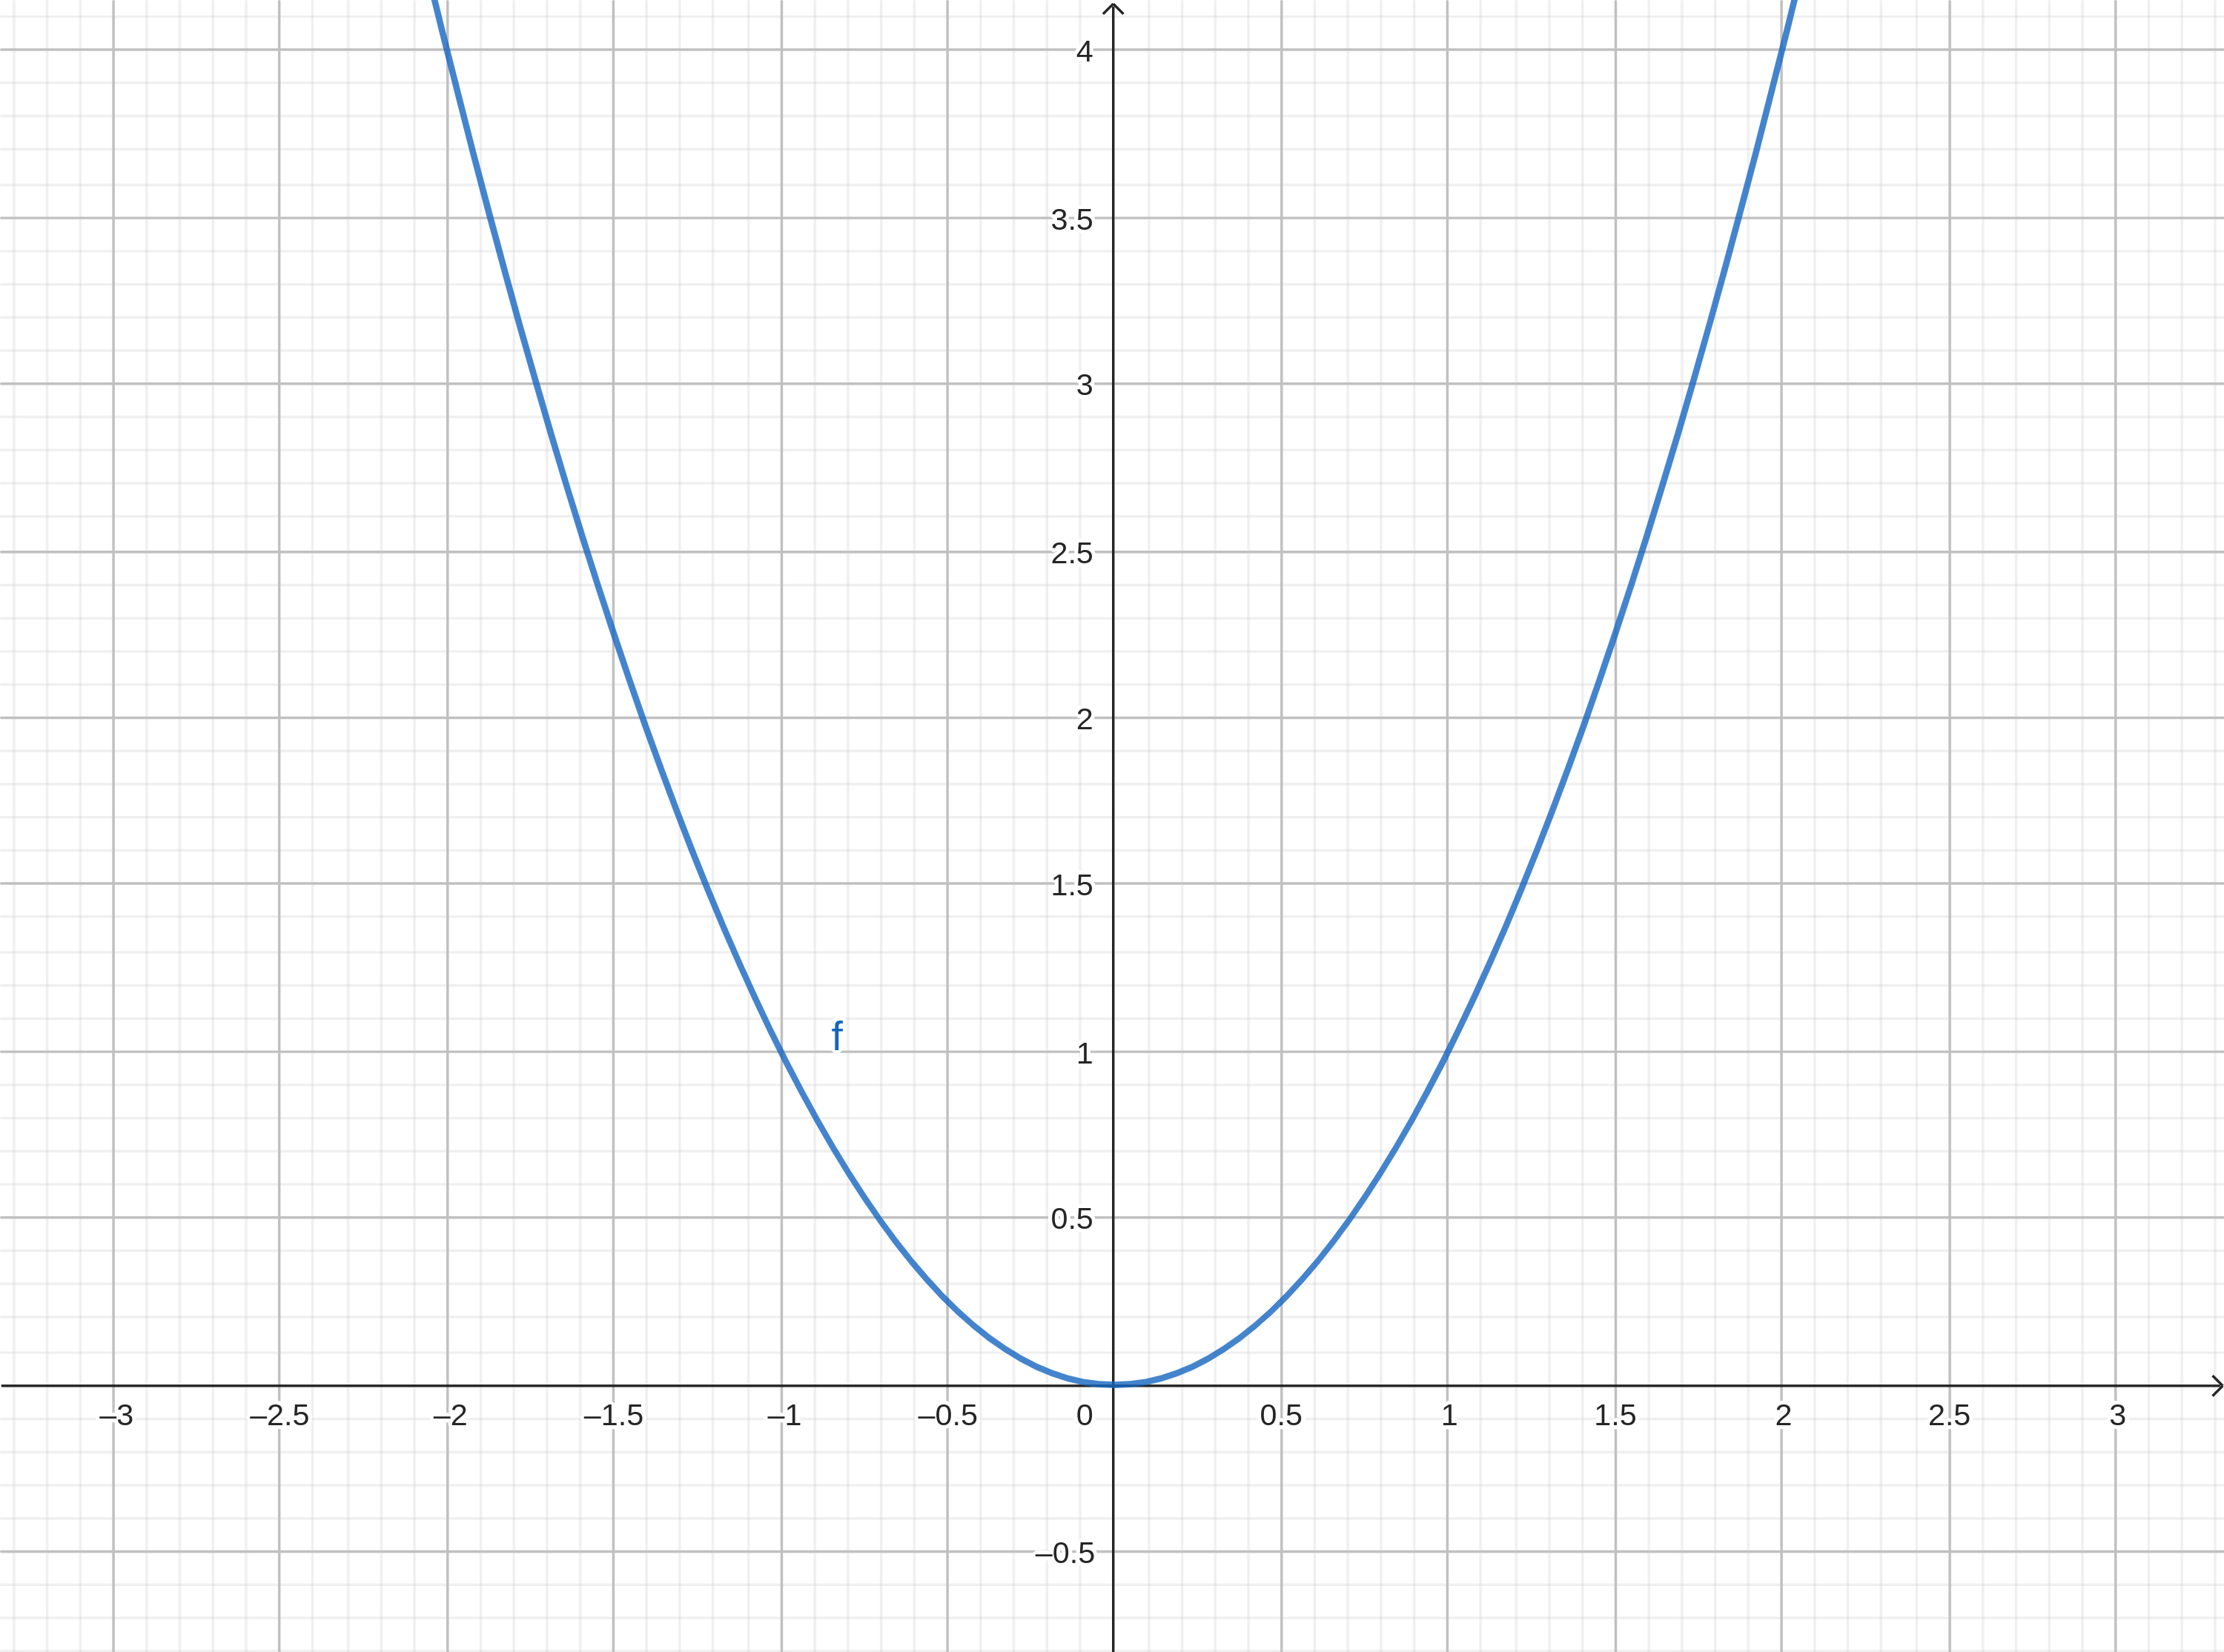
\includegraphics[width=\textwidth]{\svc/y=x^2.png}
        \caption{Parabel $y=ax^2,a\in\mathbb{R}$}
    \end{subfigure}
    \hfill
    \begin{subfigure}[b]{0.3\textwidth}
        \centering
        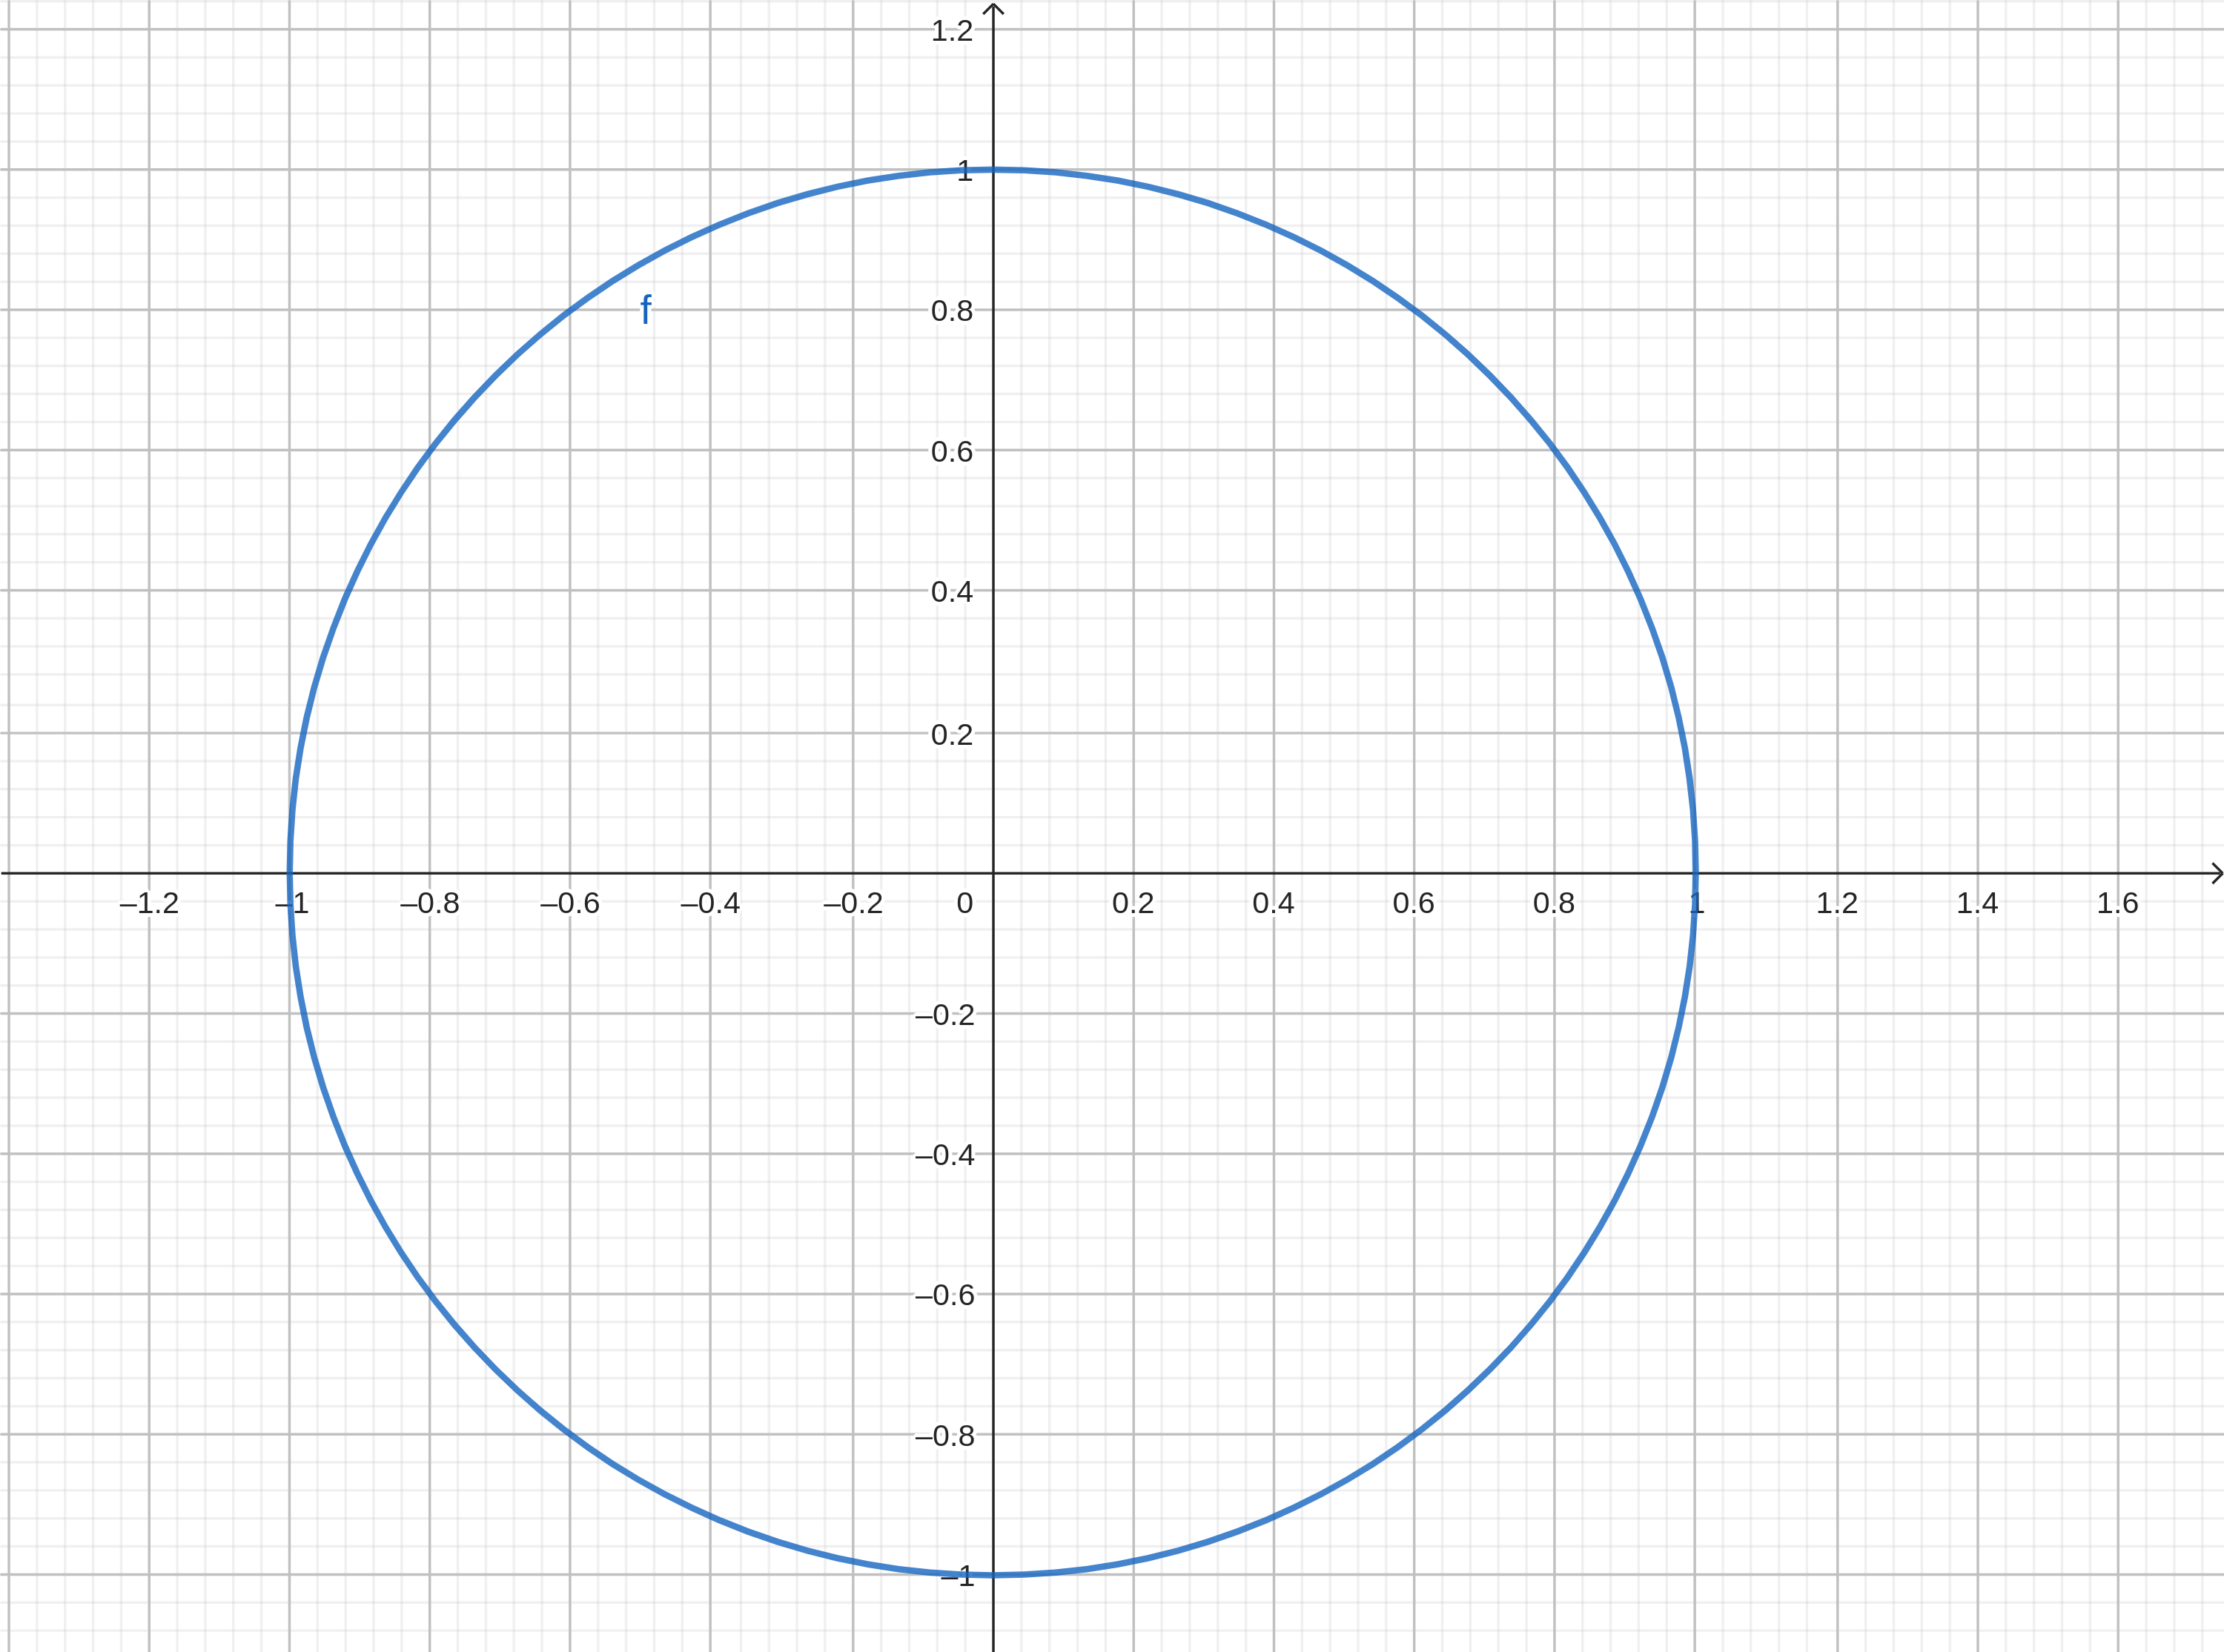
\includegraphics[width=\textwidth]{\svc/x^2+y^2=1.png}
        \caption{Ellips $ax^2+by^2=1$, $a,b>0$}
    \end{subfigure}
    \hfill
    \begin{subfigure}[b]{0.3\textwidth}
        \centering
        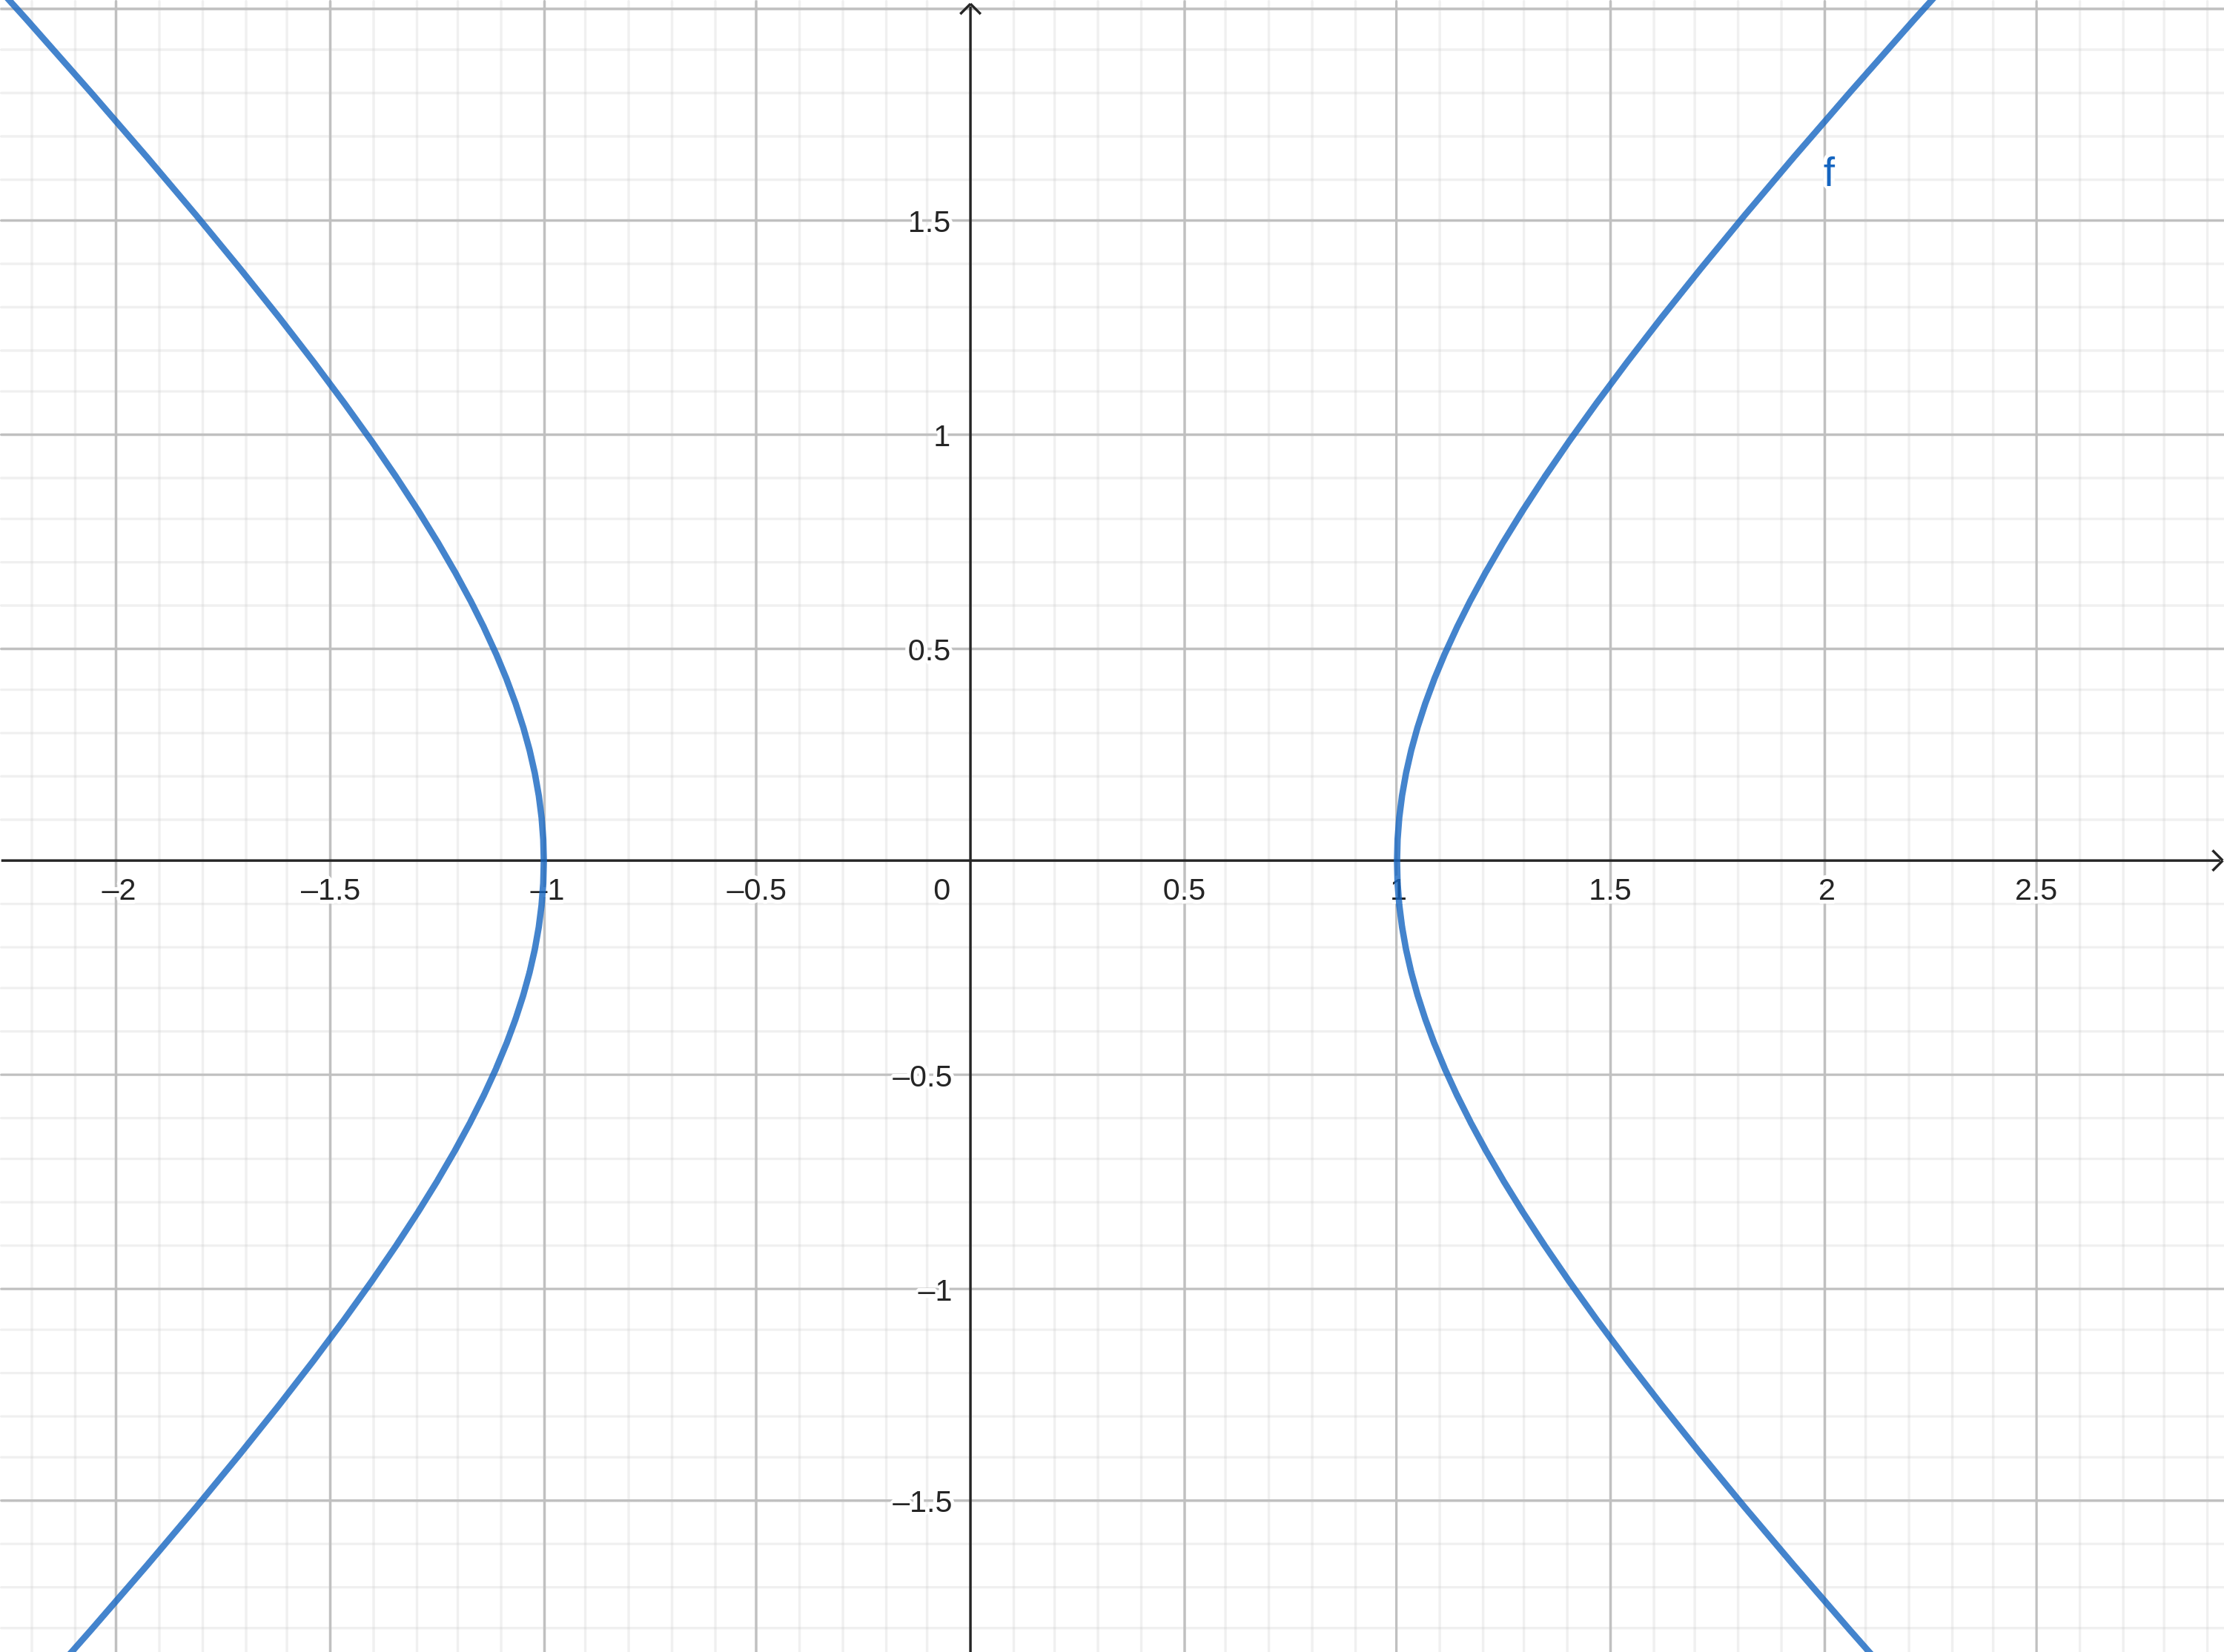
\includegraphics[width=\textwidth]{\svc/x^2-y^2=1.png}
        \caption{Hyperbel $ax^2-by^2=1$, $a,b>0$}
    \end{subfigure}
    \hfill
    \begin{subfigure}[b]{0.3\textwidth}
        \centering
        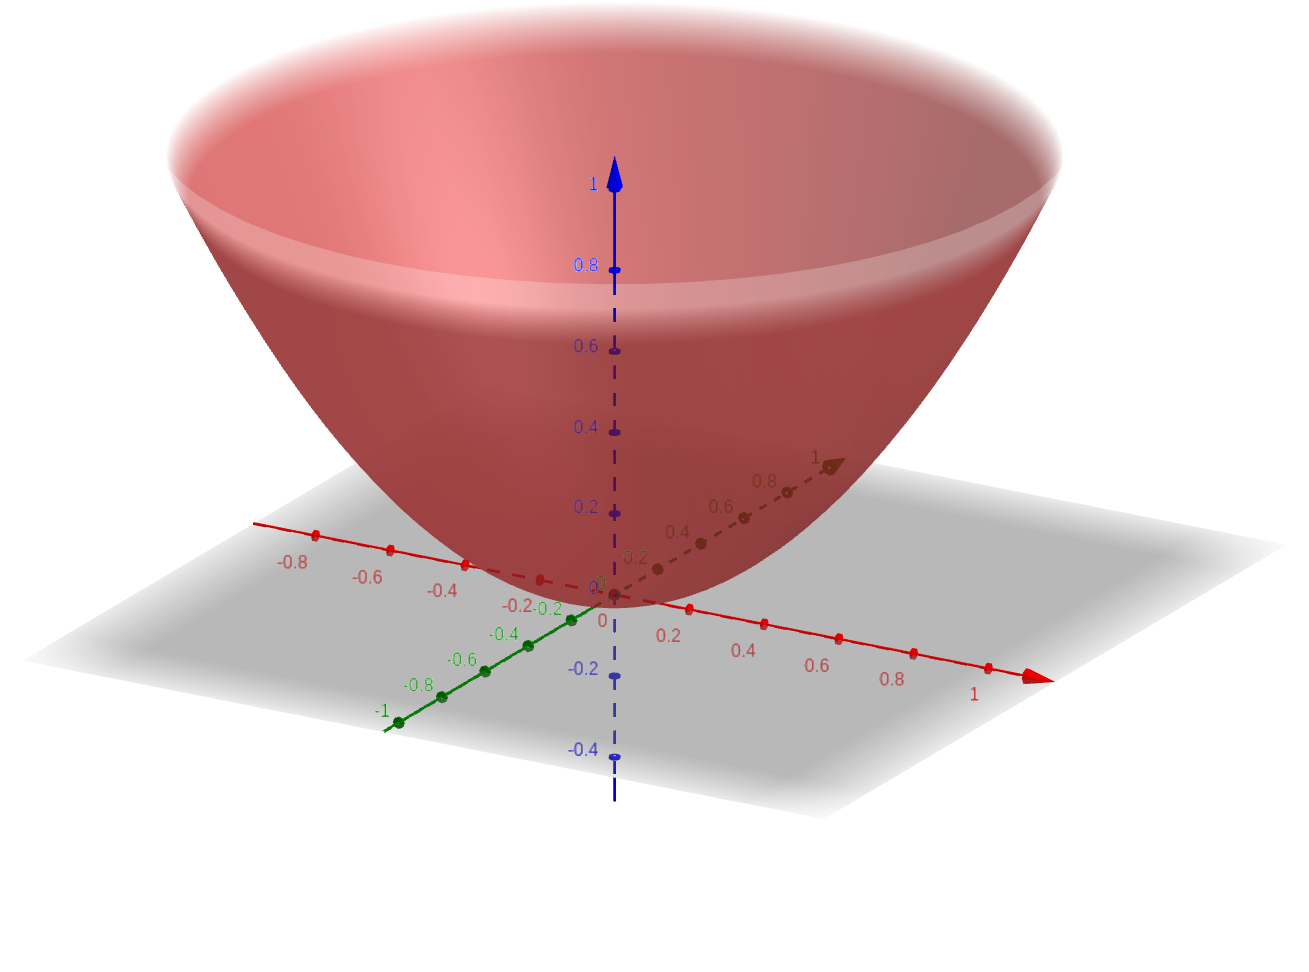
\includegraphics[width=\textwidth]{\svc/x^2+y^2=z.png}
        \caption{Elliptisk paraboid $z=ax^2+bx^2$, $a,b>0$}
    \end{subfigure}
    \hfill
    \begin{subfigure}[b]{0.3\textwidth}
        \centering
        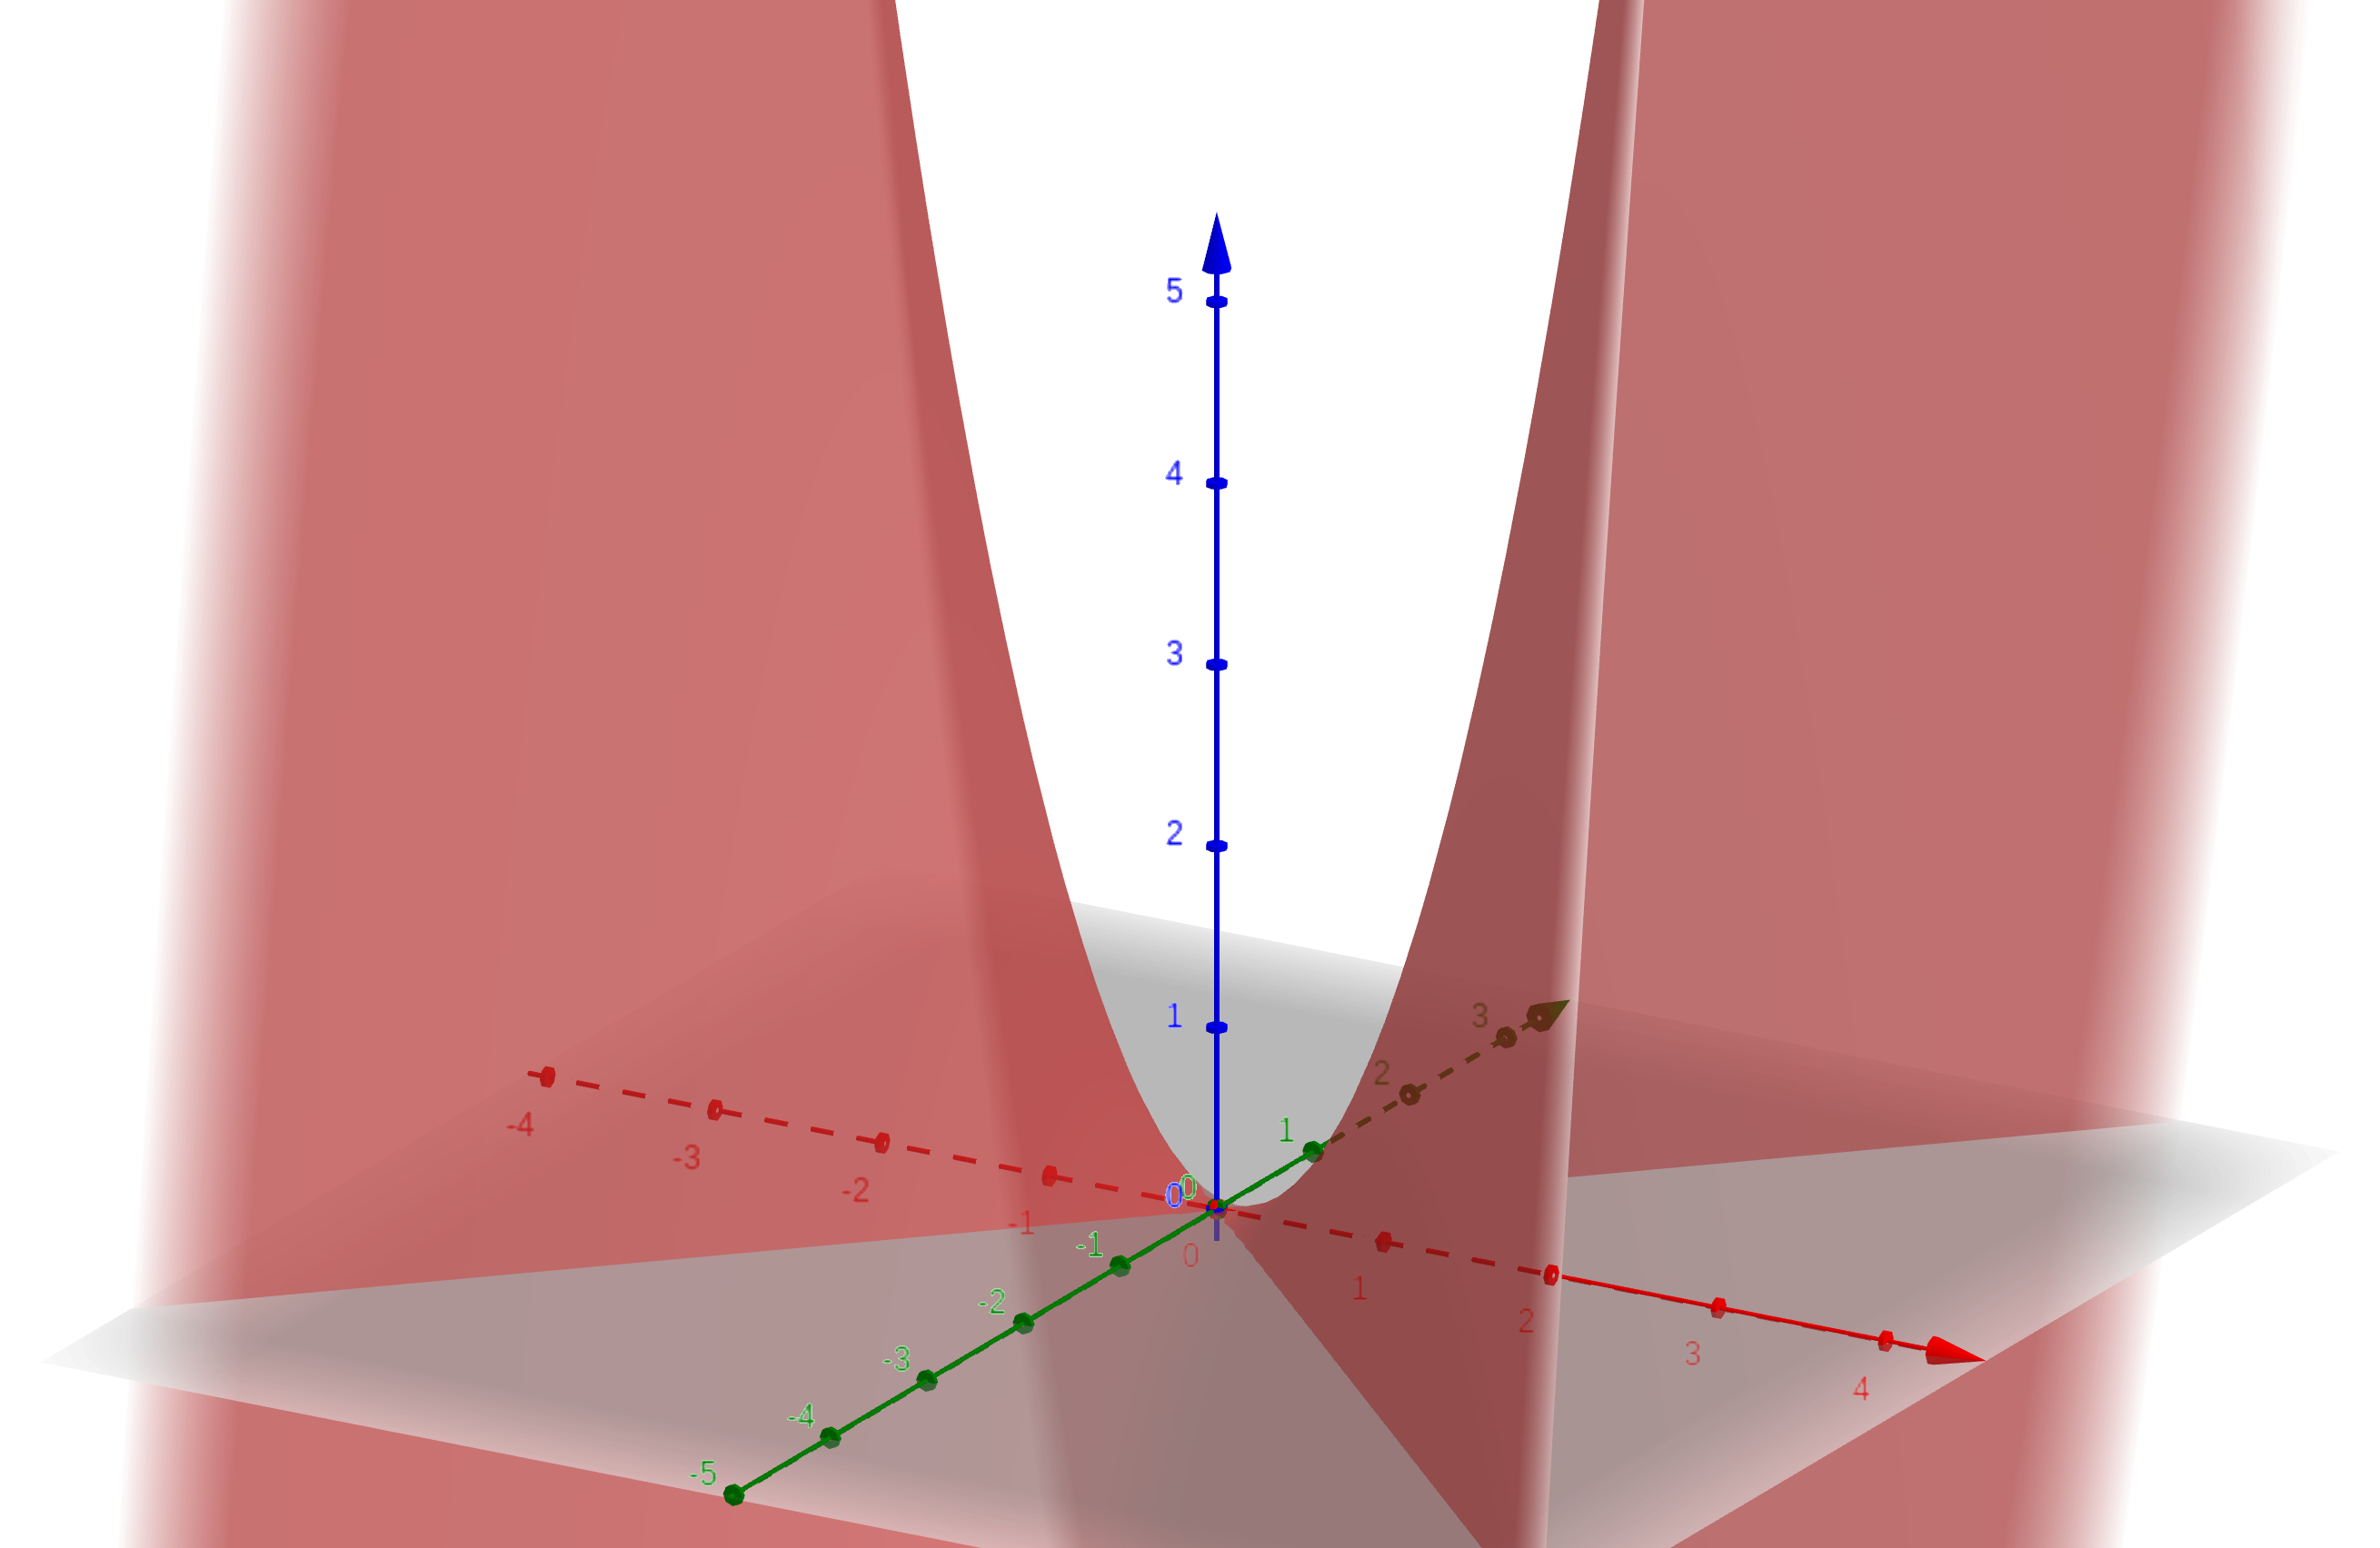
\includegraphics[width=\textwidth]{\svc/z=x^2-y^2.png}
        \caption{Hyperbolisk parabolid $z=ax^2-by^2$, $a,b>0$}
    \end{subfigure}
    \hfill
    \begin{subfigure}[b]{0.3\textwidth}
        \centering
        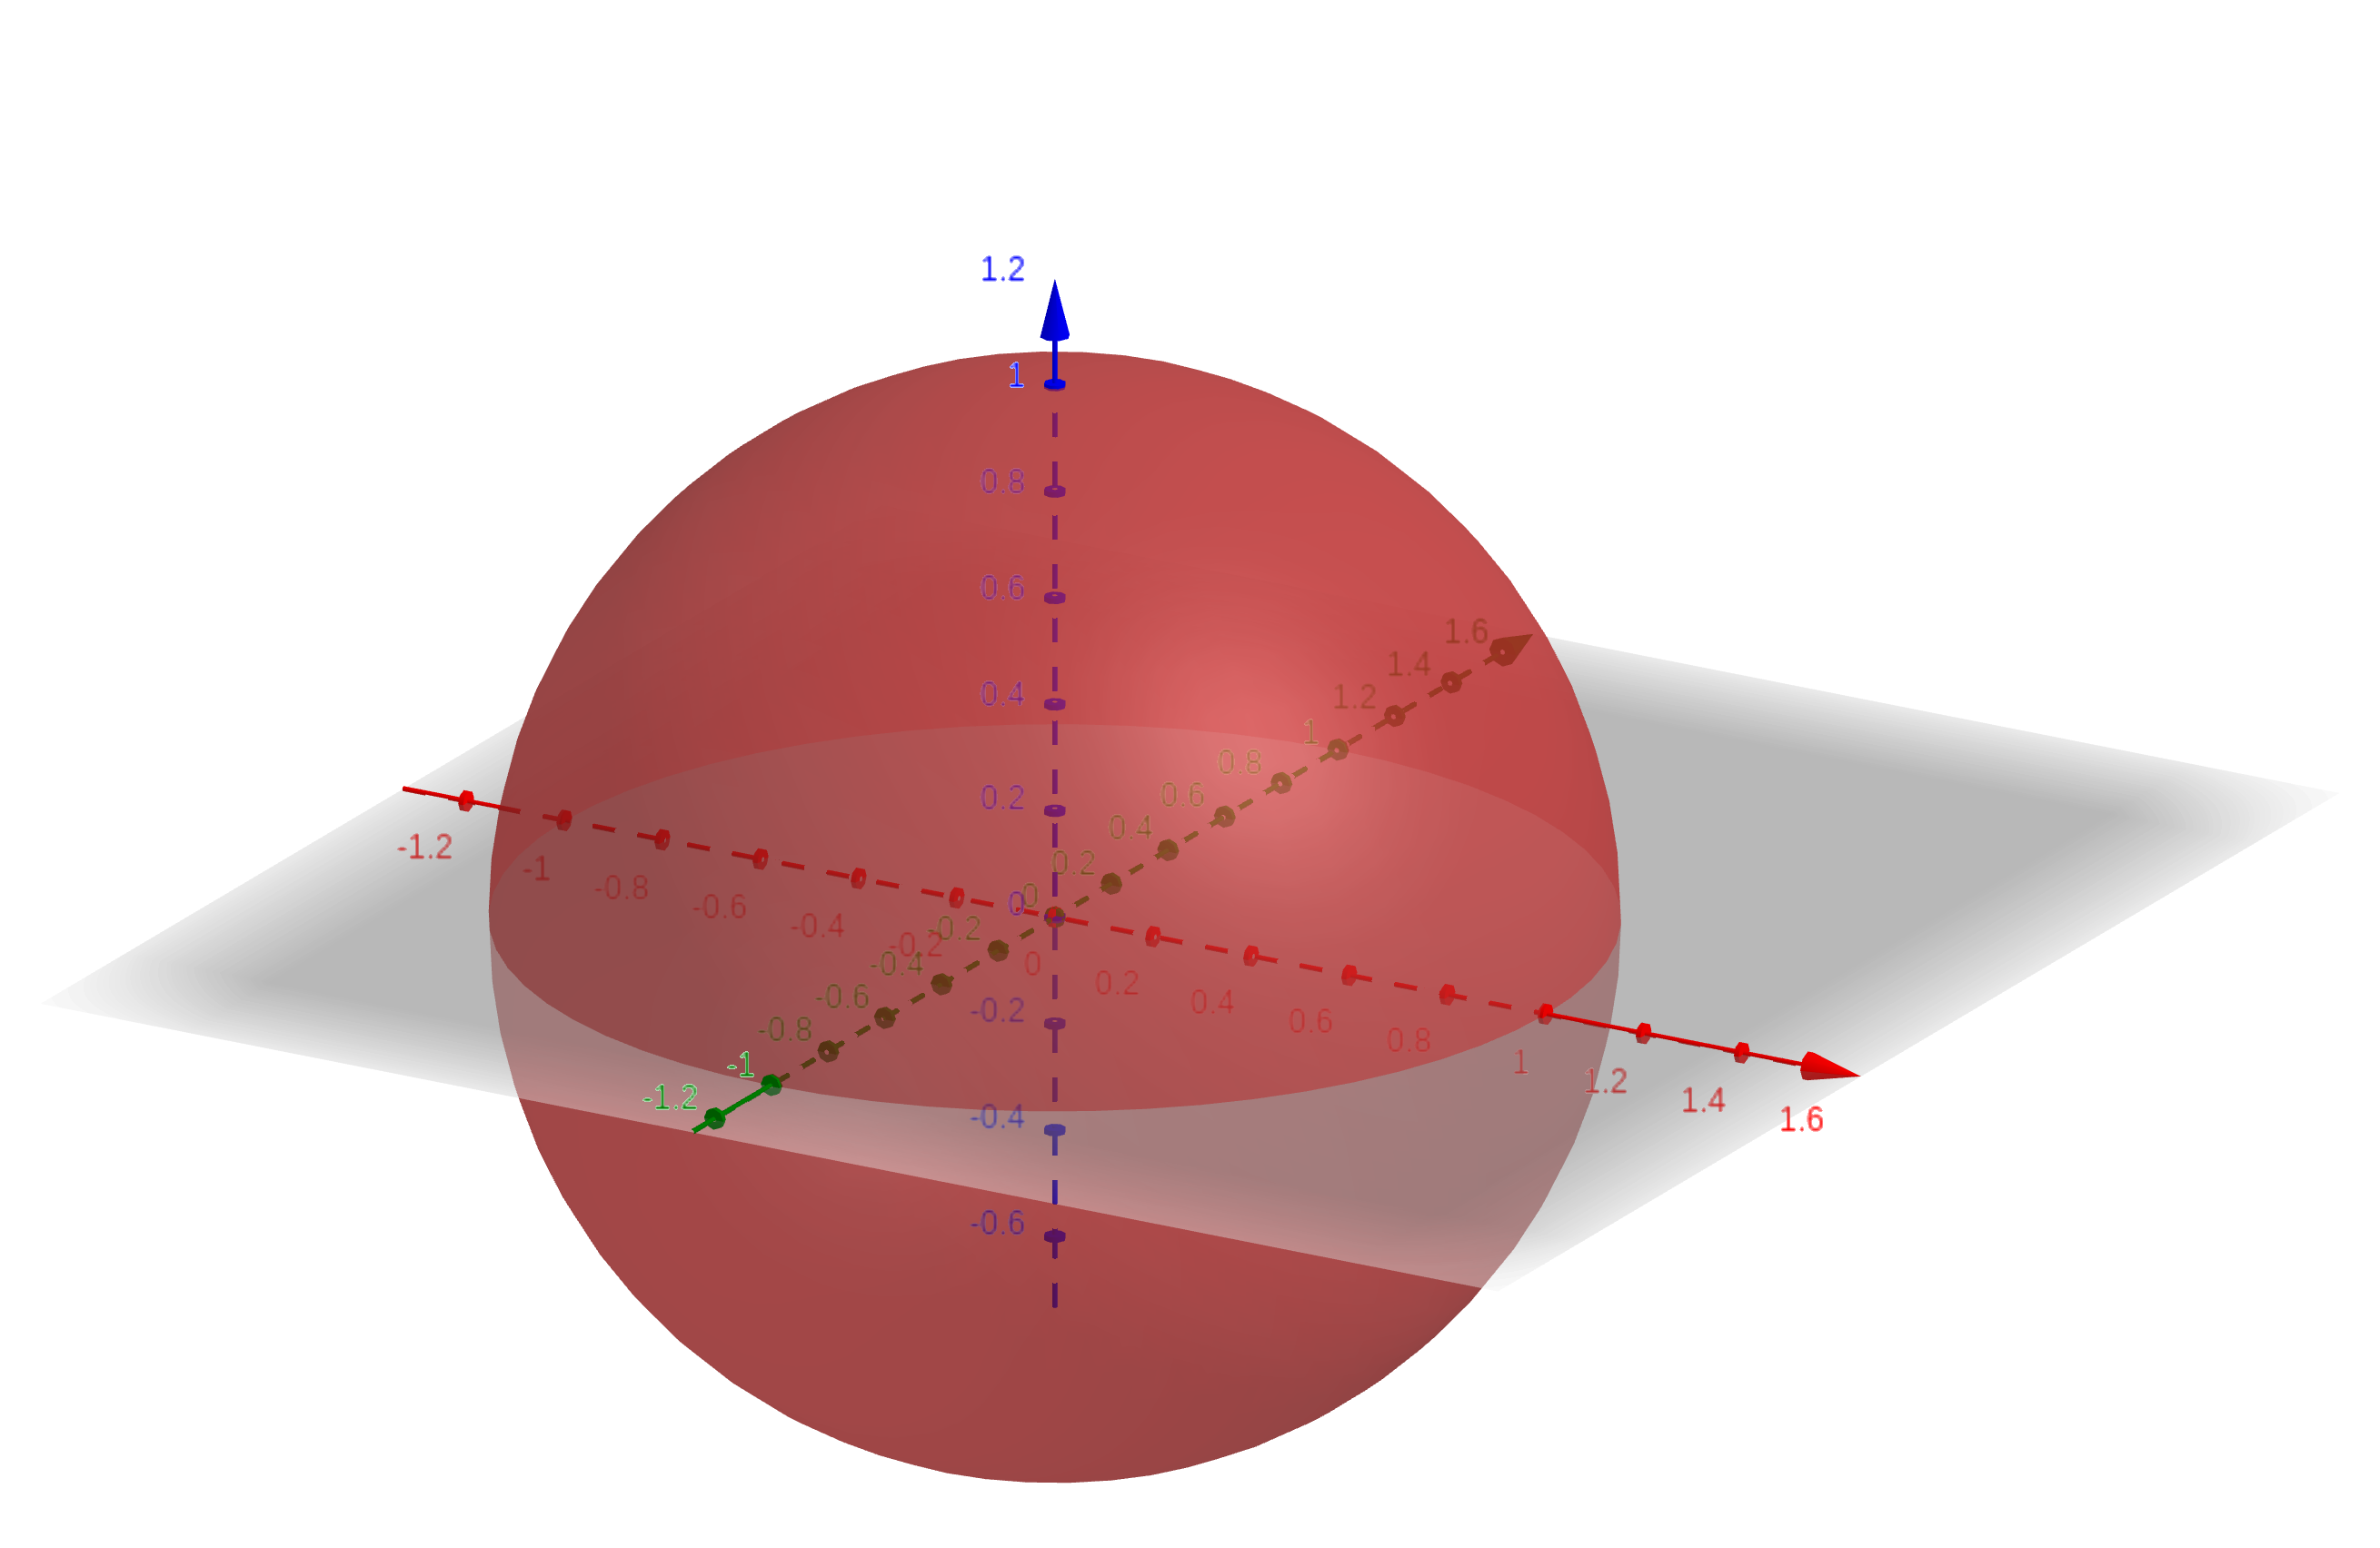
\includegraphics[width=\textwidth]{\svc/x^2+y^2+z^2=1.png}
        \caption{Ellipsoid $ax^2+by^2+cz^2=1$, $a,b,c>0$}
    \end{subfigure}
    \hfill
    \begin{subfigure}[b]{0.3\textwidth}
        \centering
        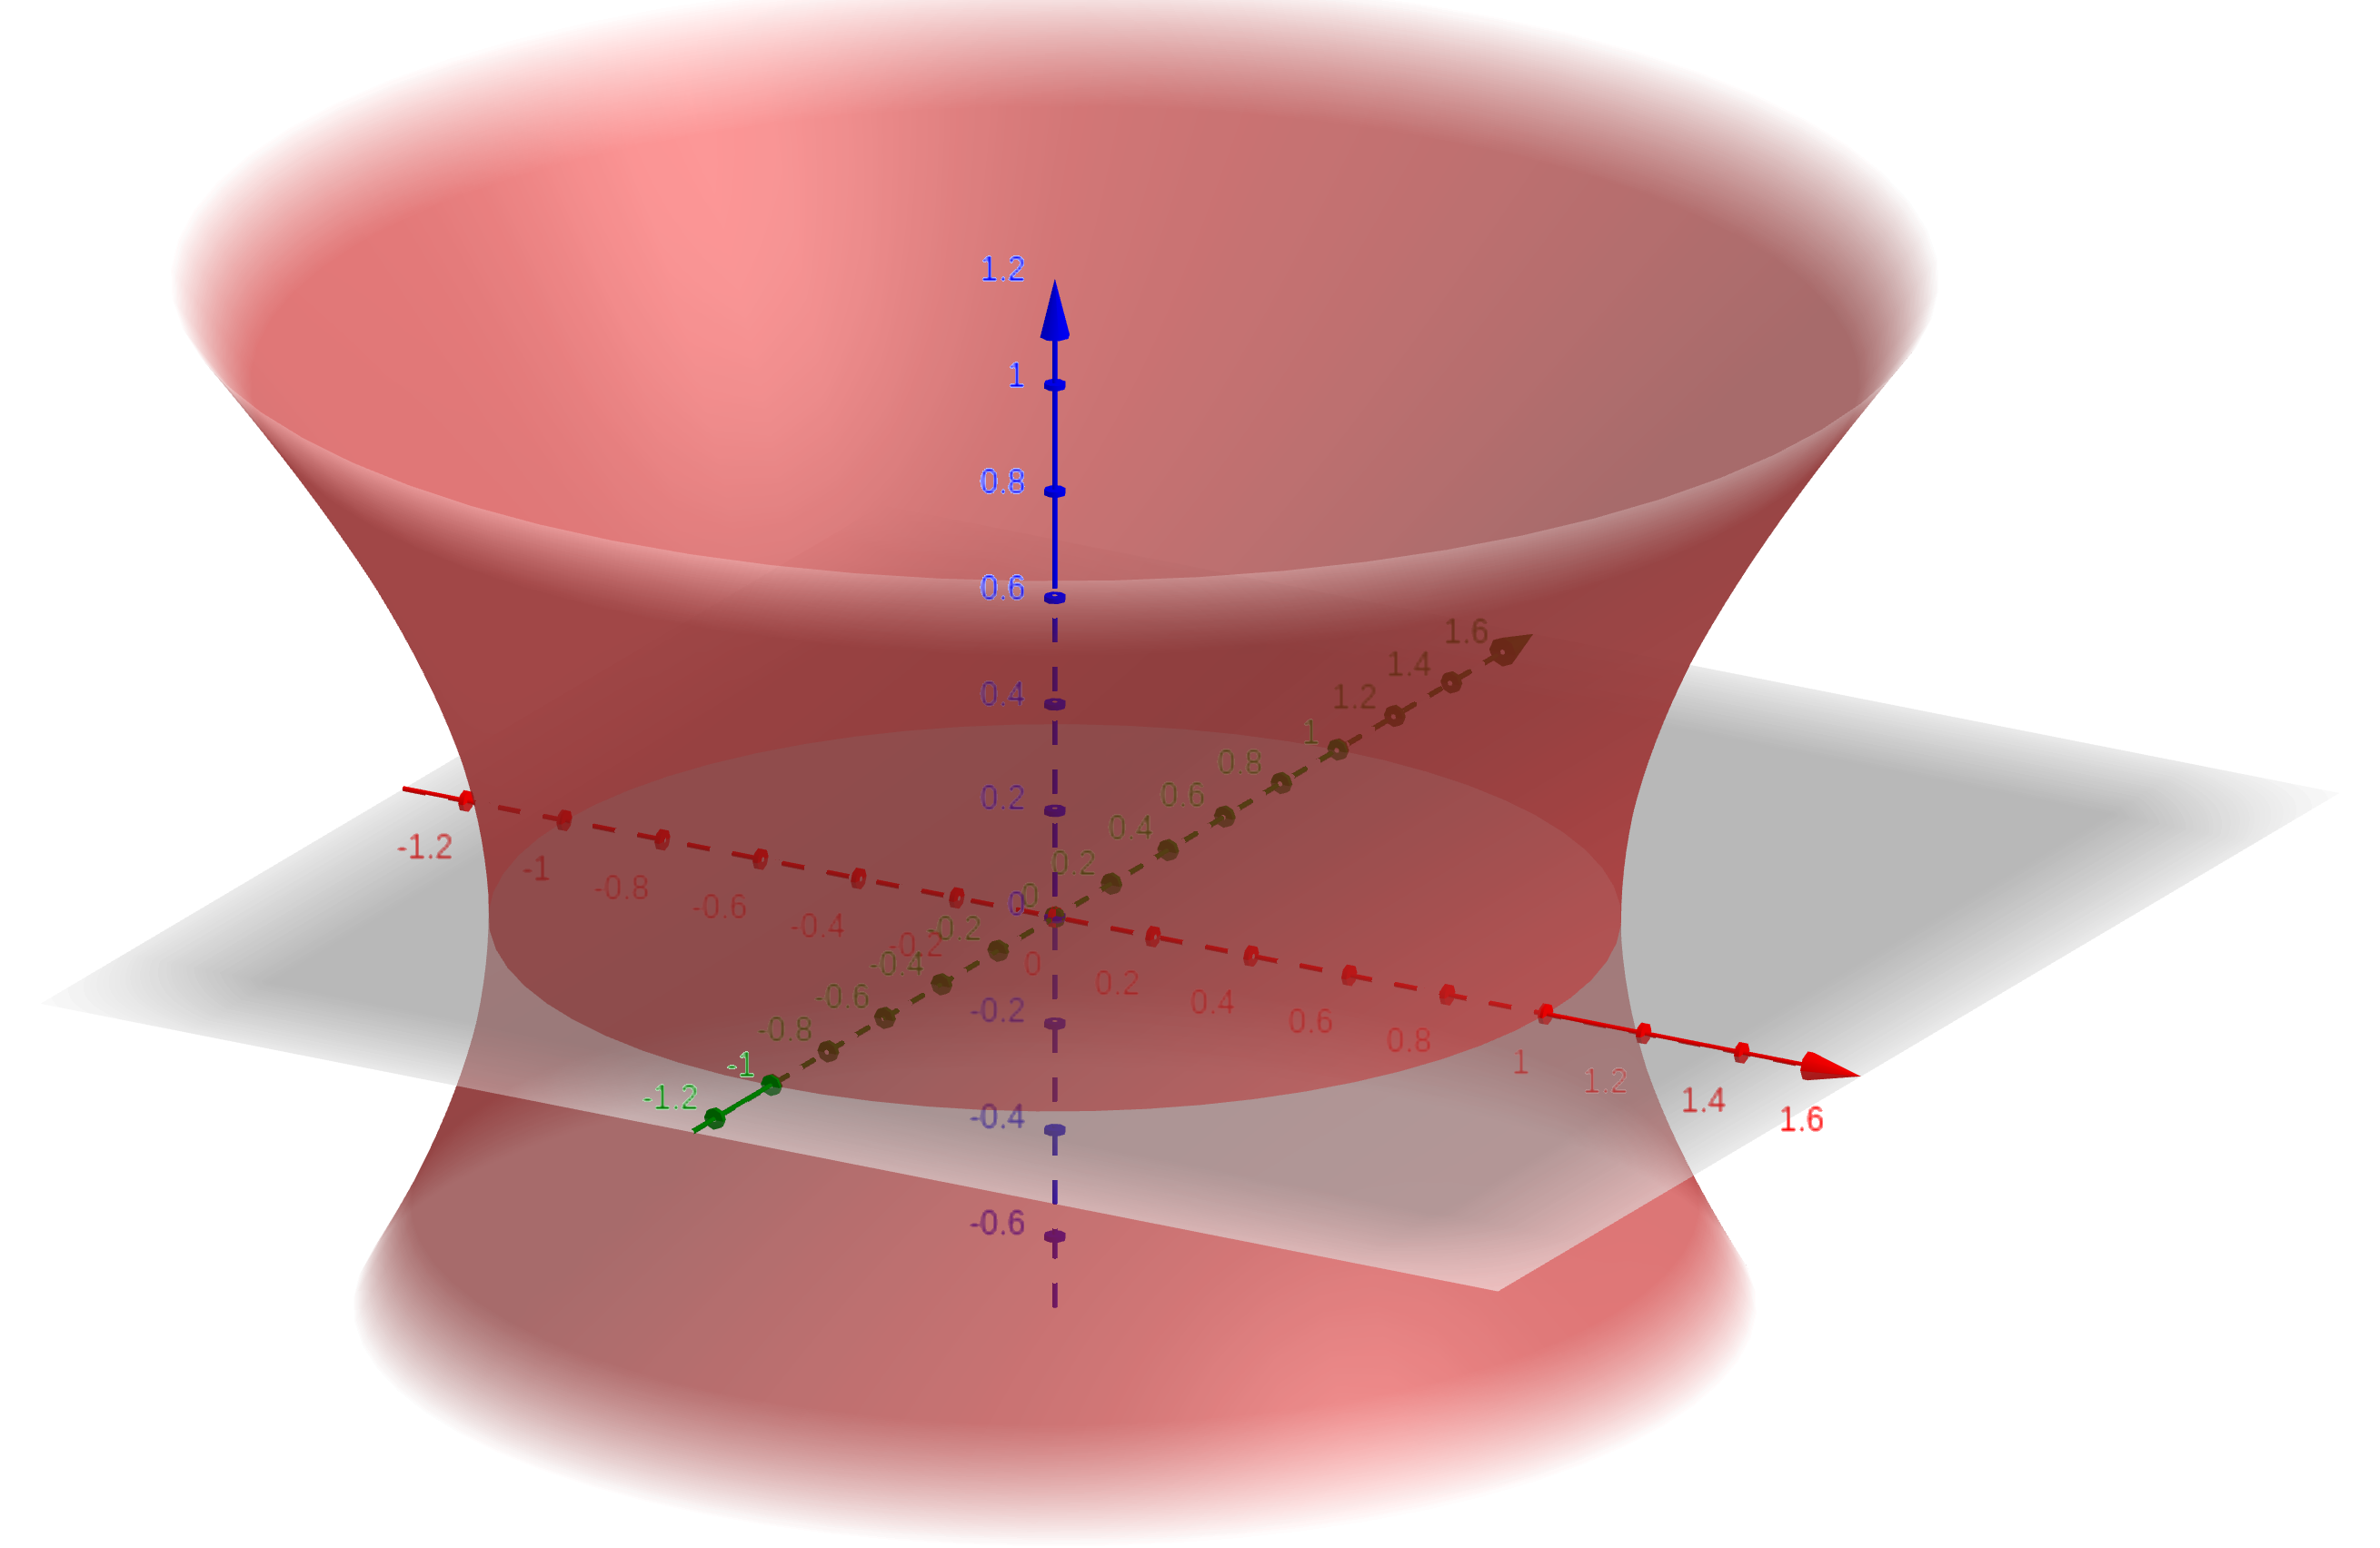
\includegraphics[width=\textwidth]{\svc/x^2+y^2-z^2=1.png}
        \caption{Enmantlad hyperboloid $ax^2+by^2-cz^2=1$, $a,b,c>0$}
    \end{subfigure}
    \hfill
    \begin{subfigure}[b]{0.3\textwidth}
        \centering
        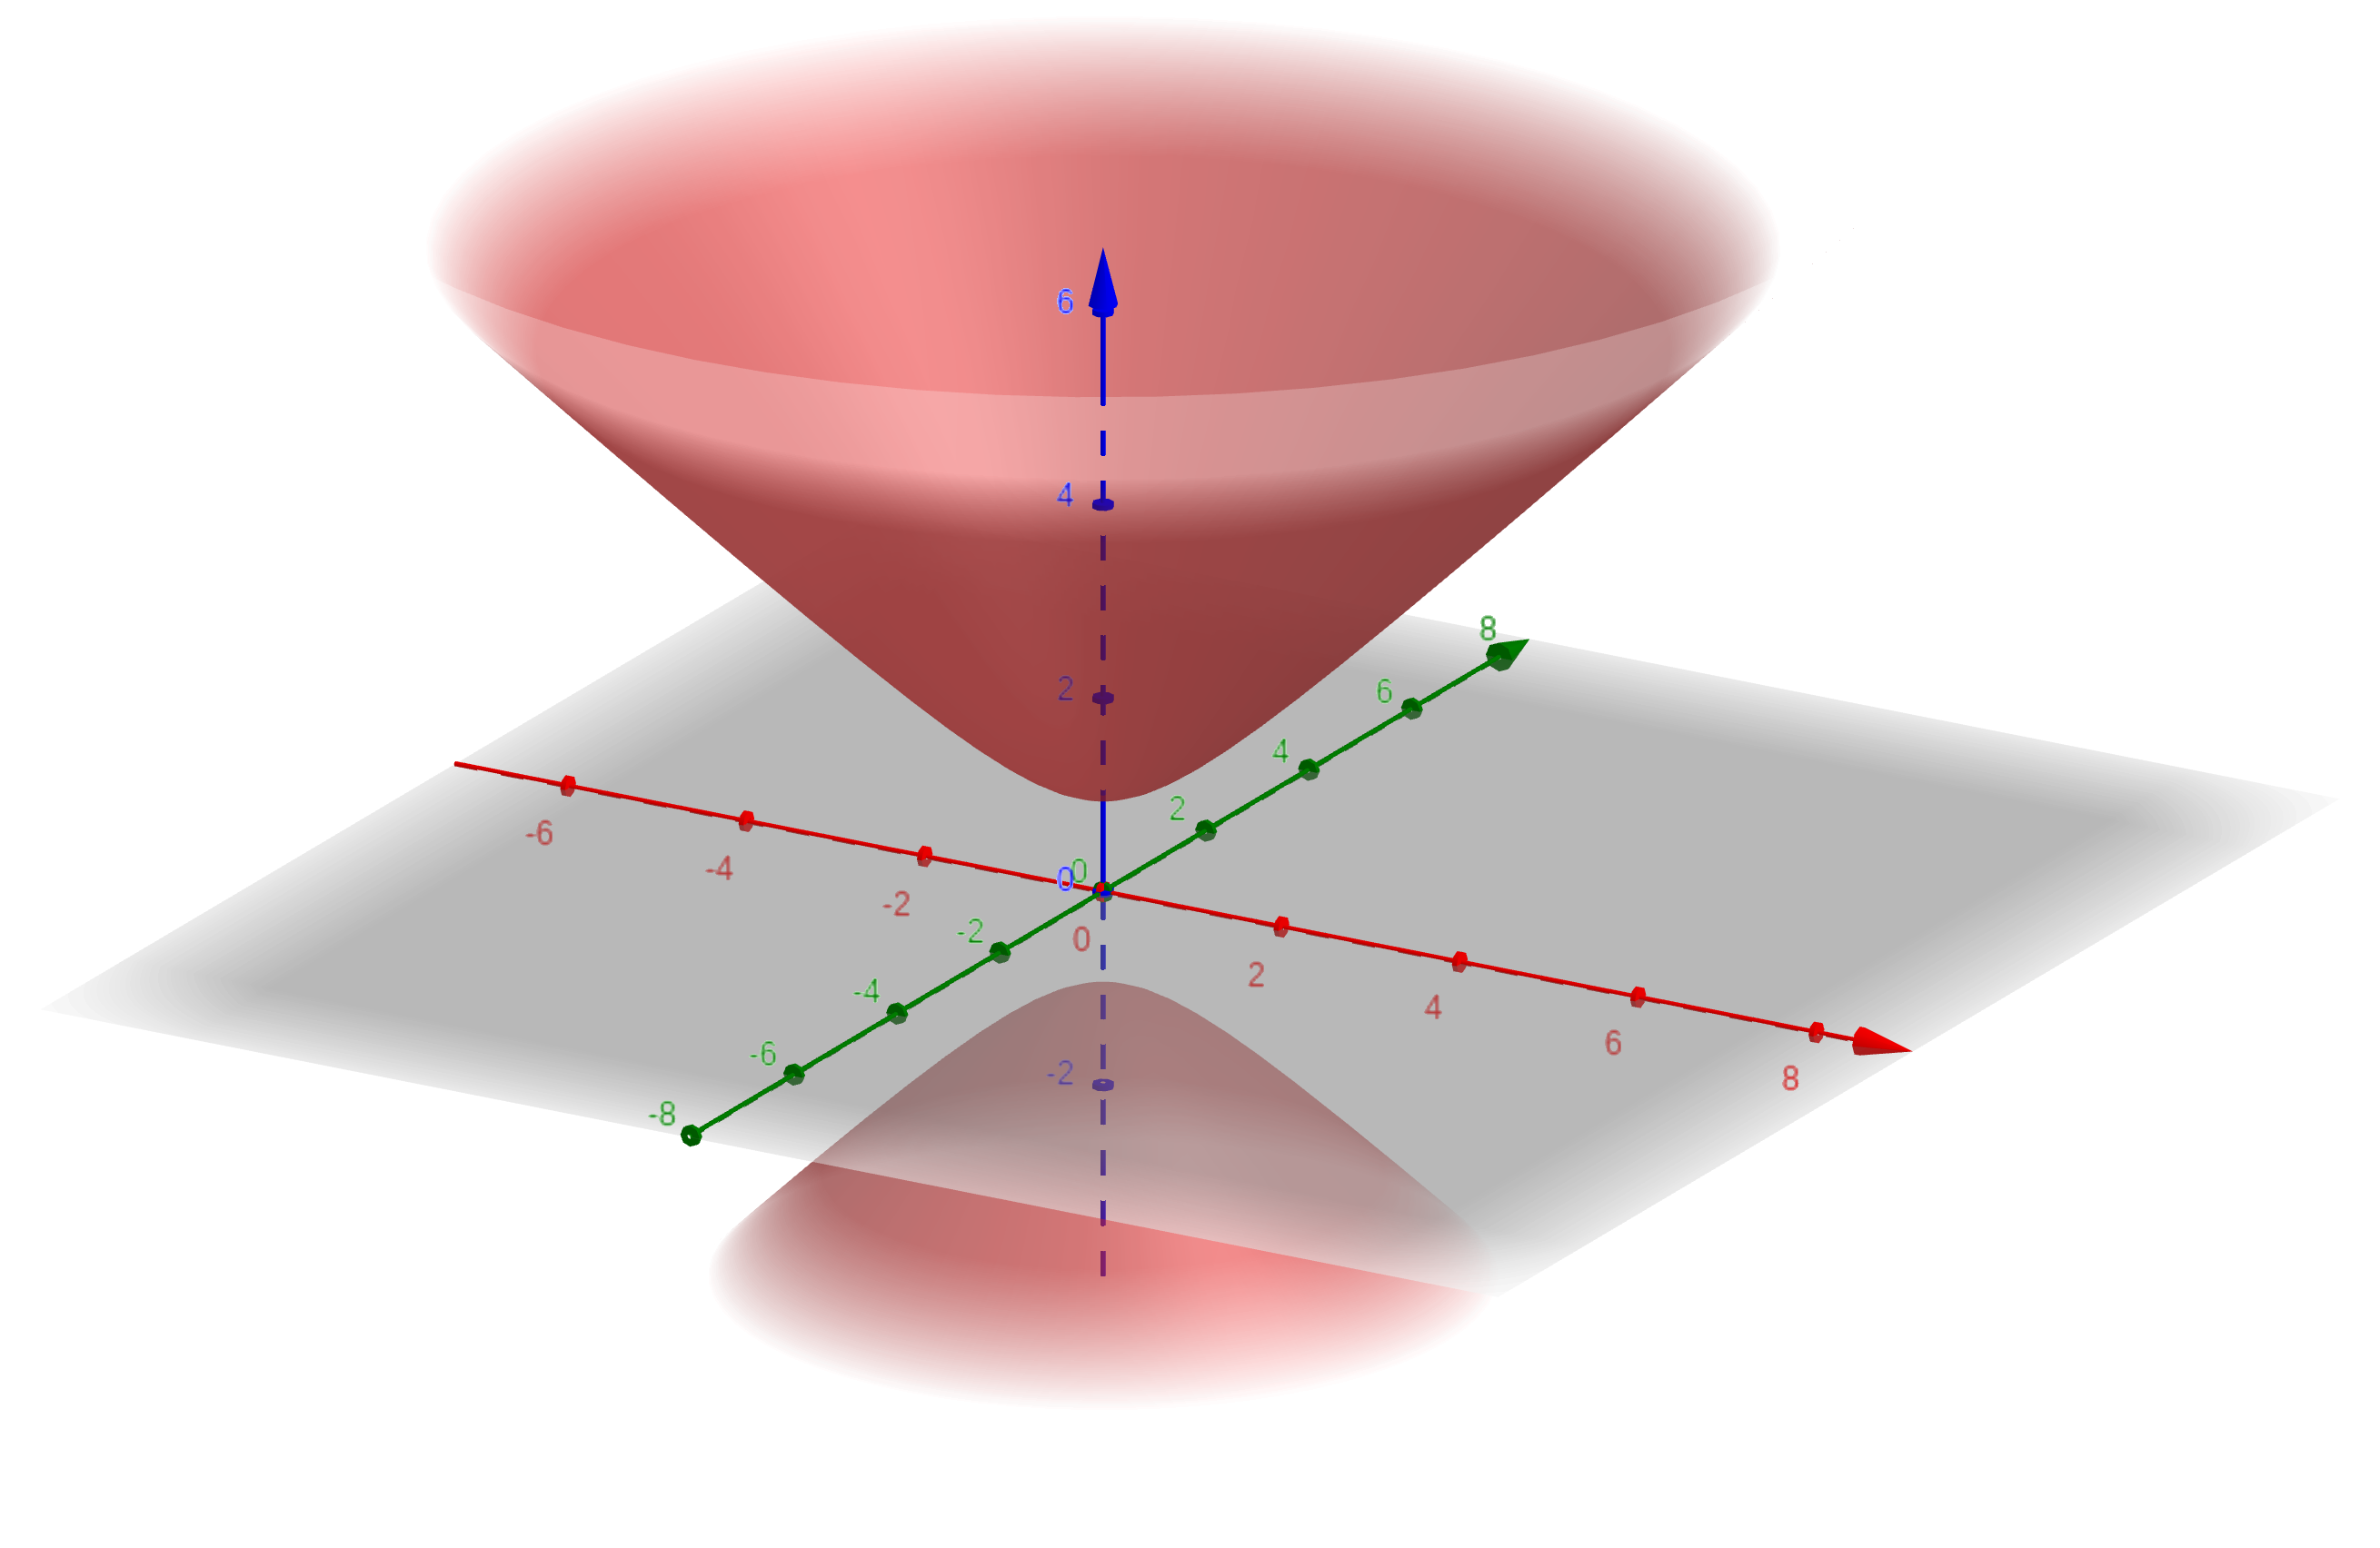
\includegraphics[width=\textwidth]{\svc/-x^2-y^2+z^2=1.png}
        \caption{Tvåmantlad hyperboloid $-ax^2-by^2+cz^2=1$, $a,b,c>0$}
    \end{subfigure}
    \hfill
    \begin{subfigure}[b]{0.3\textwidth}
        \centering
        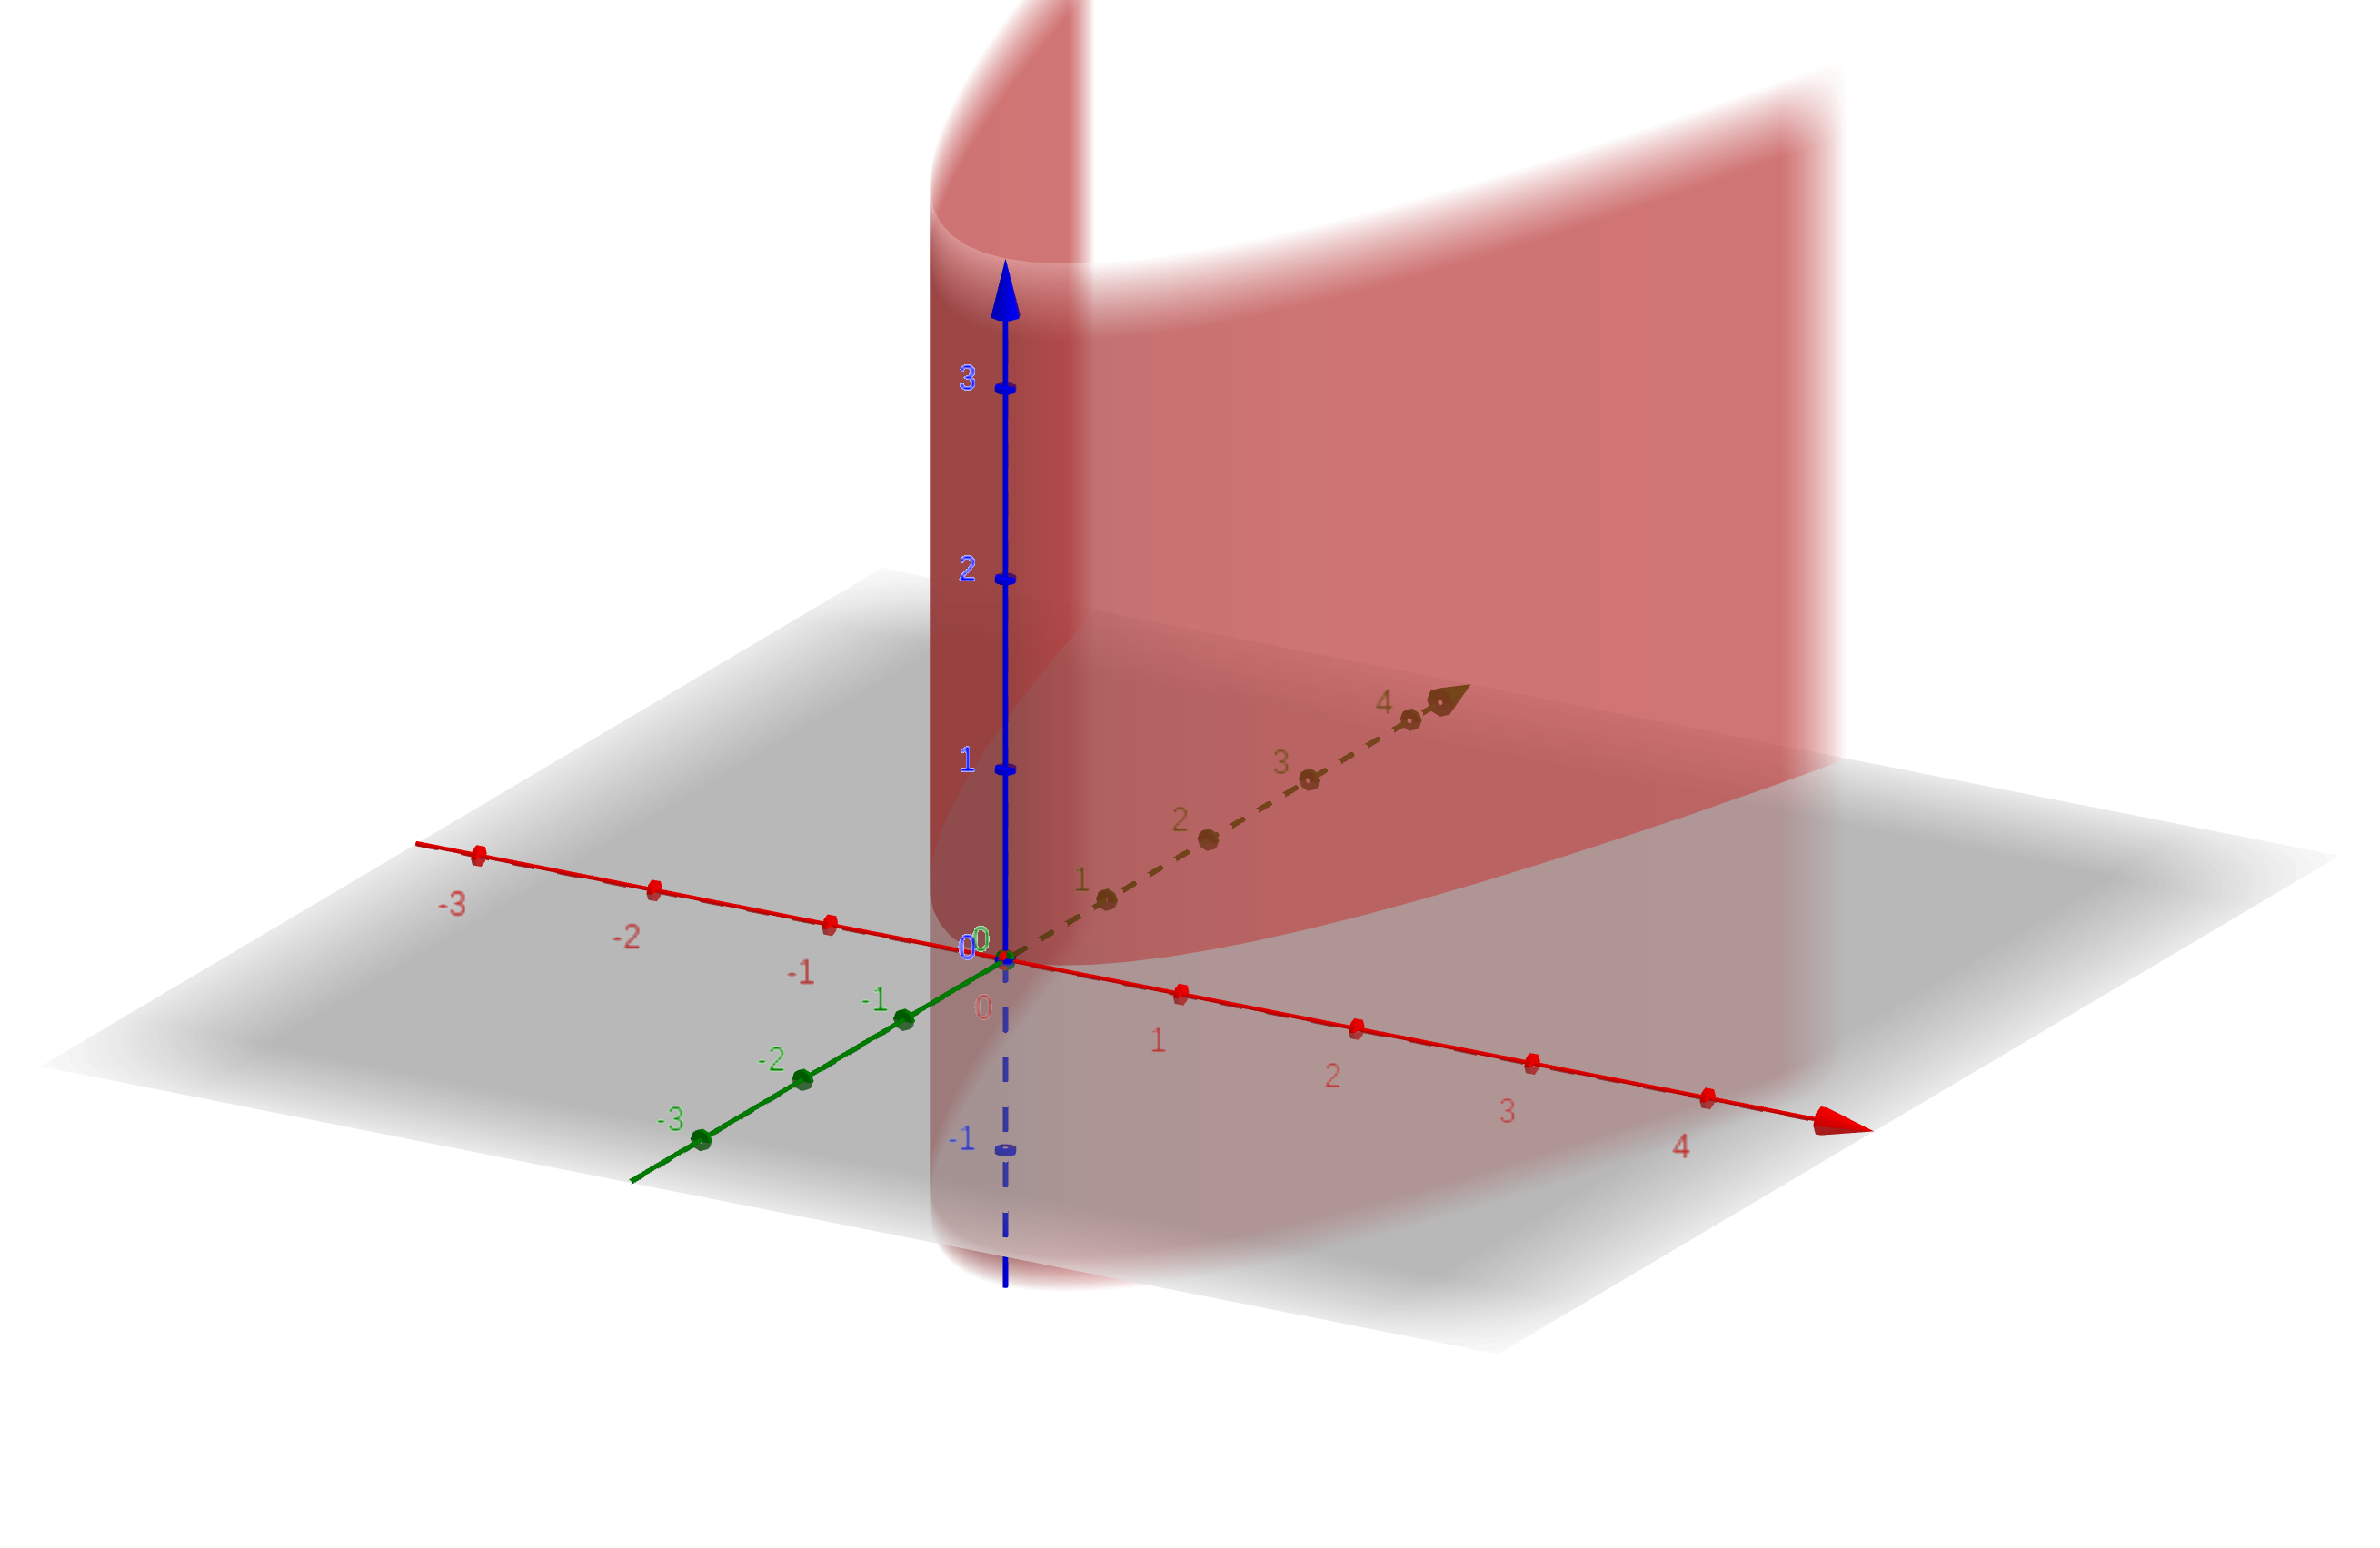
\includegraphics[width=\textwidth]{\svc/y=x^2(3d).png}
        \caption{Parabolisk cylinder $y=ax^2$, $a>0$}
    \end{subfigure}
    \hfill
    \begin{subfigure}[b]{0.3\textwidth}
        \centering
        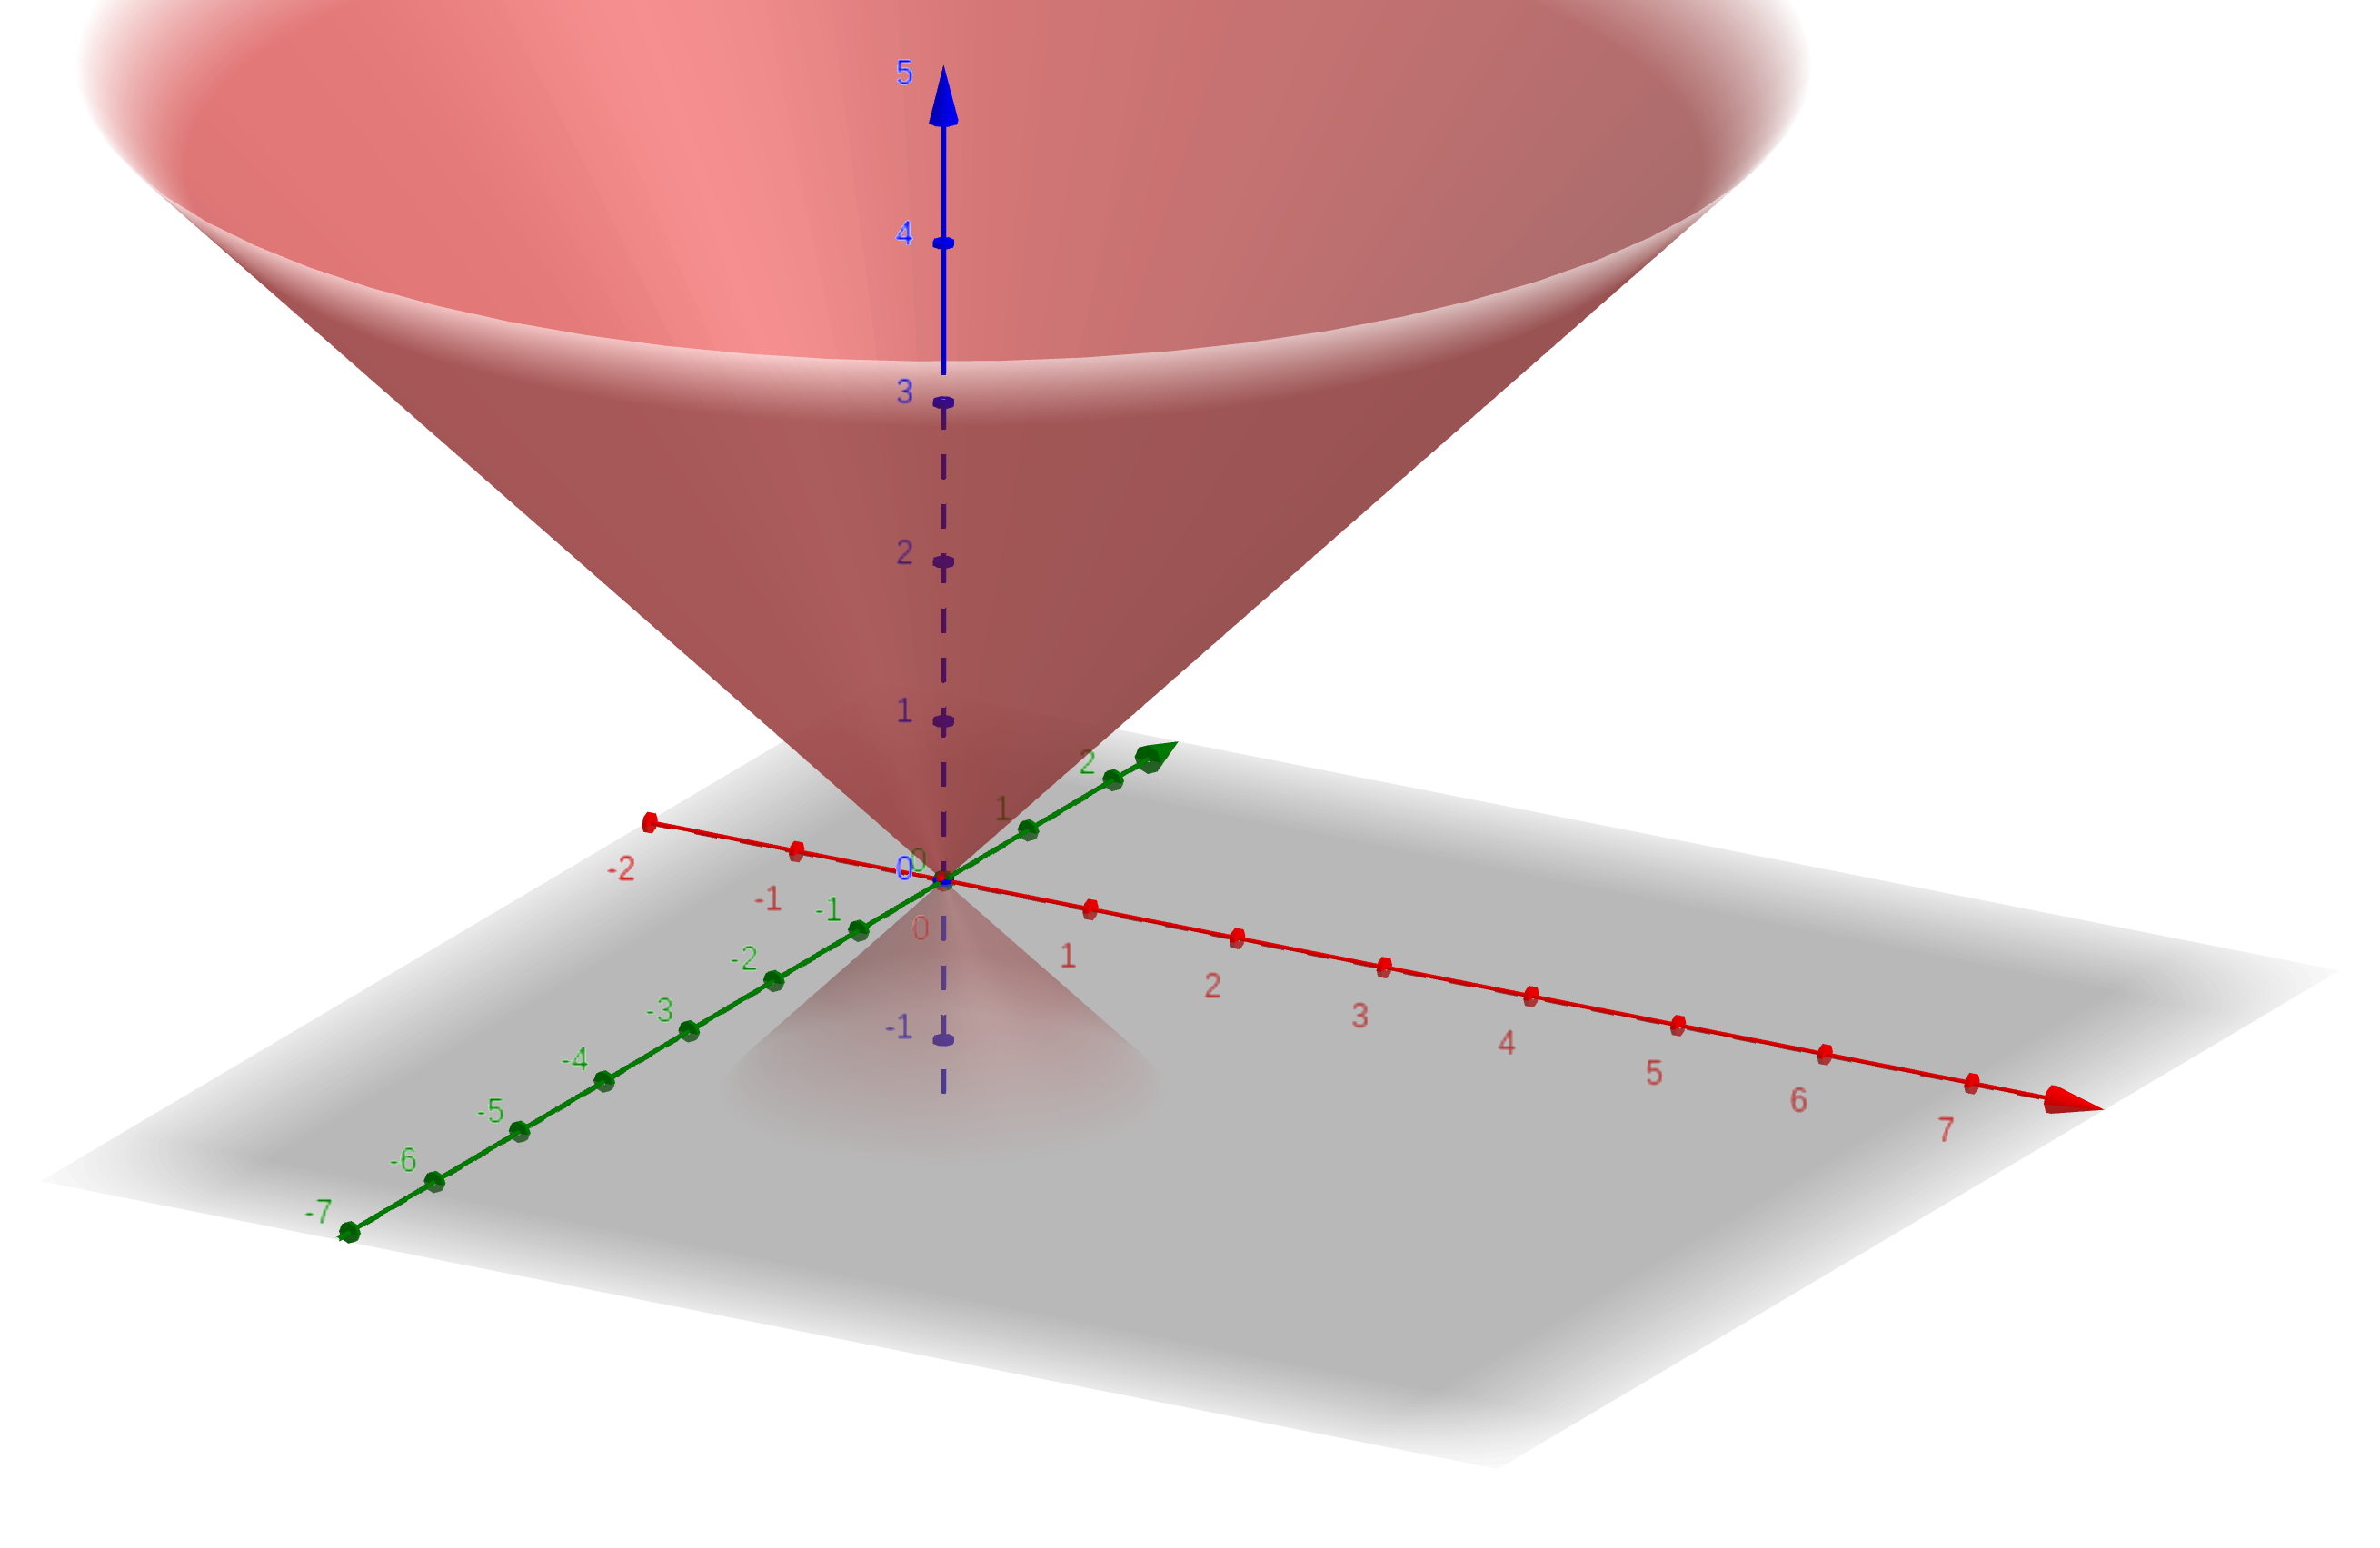
\includegraphics[width=\textwidth]{\svc/x^2+y^2-z^2=0.png}
        \caption{Eliptisk kon $ax^2+by^2+cz^2=0$, $a,b,c>0$}
    \end{subfigure}
    \hfill
    \begin{subfigure}[b]{0.3\textwidth}
        \centering
        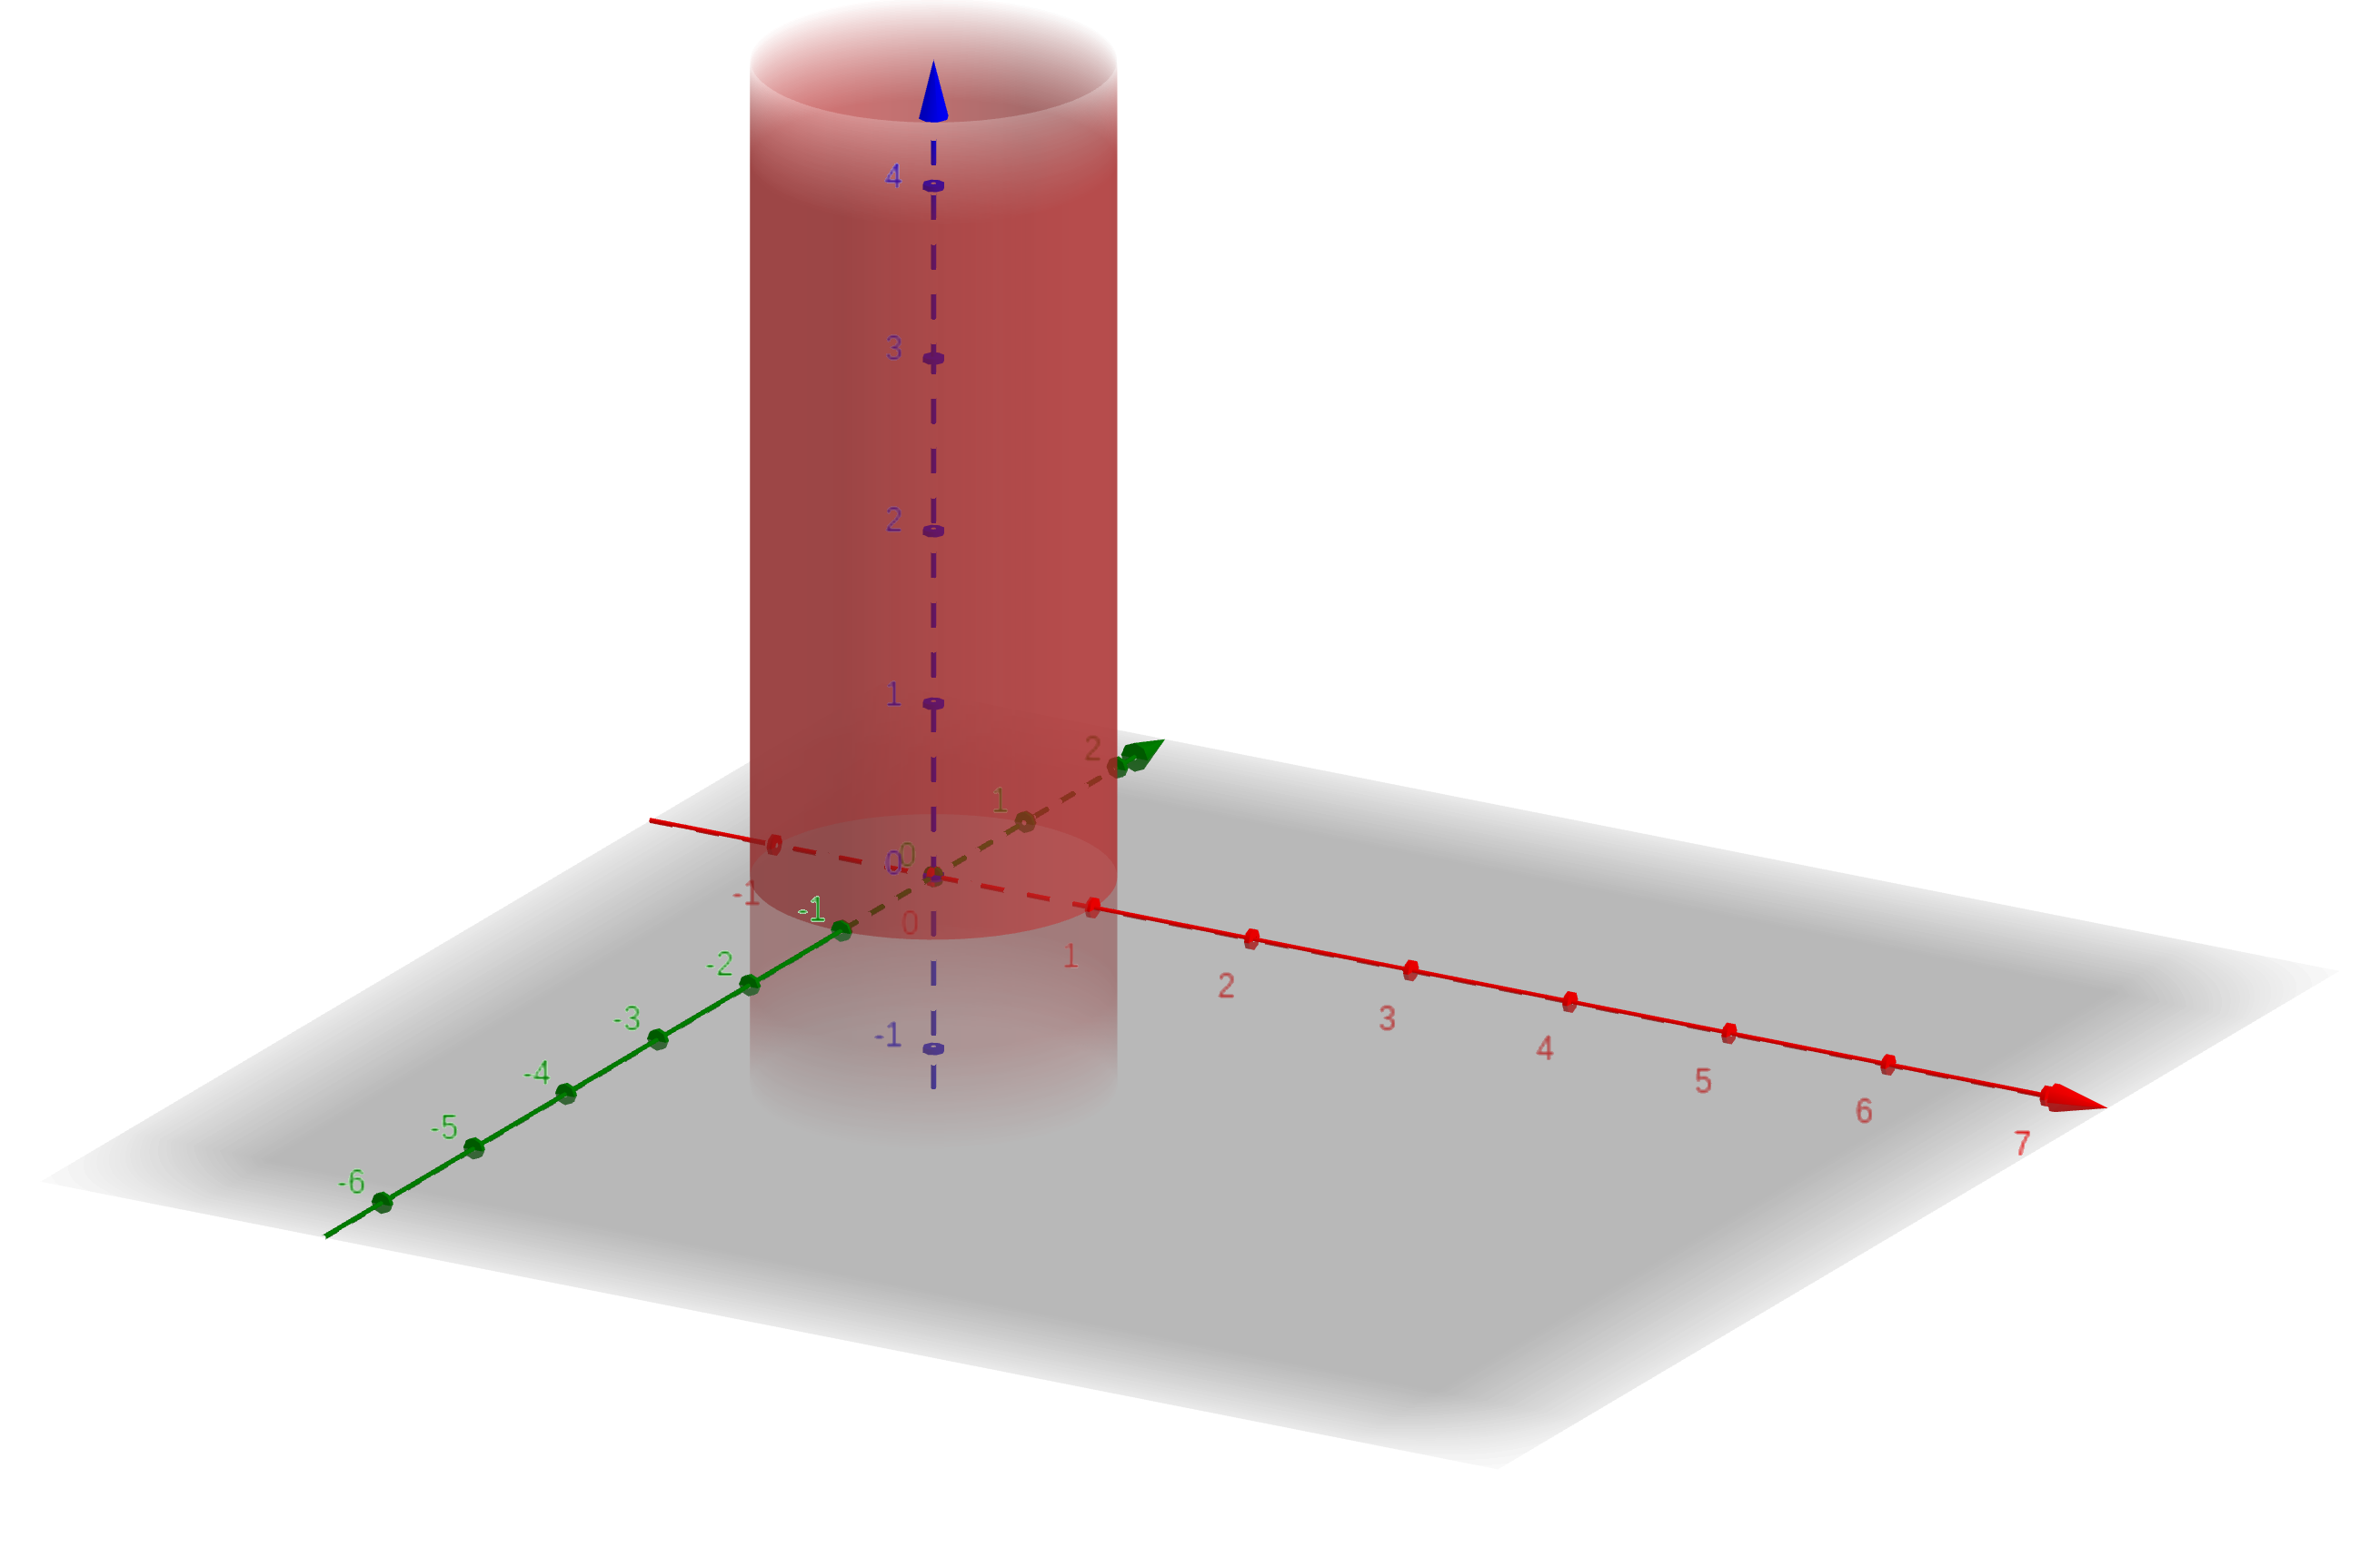
\includegraphics[width=\textwidth]{\svc/x^2+y^2=1(3d).png}
        \caption{Eliptisk cylinder $ax^2+by^2=1$, $a,b>0$}
    \end{subfigure}
    \hfill
    \begin{subfigure}[b]{0.3\textwidth}
        \centering
        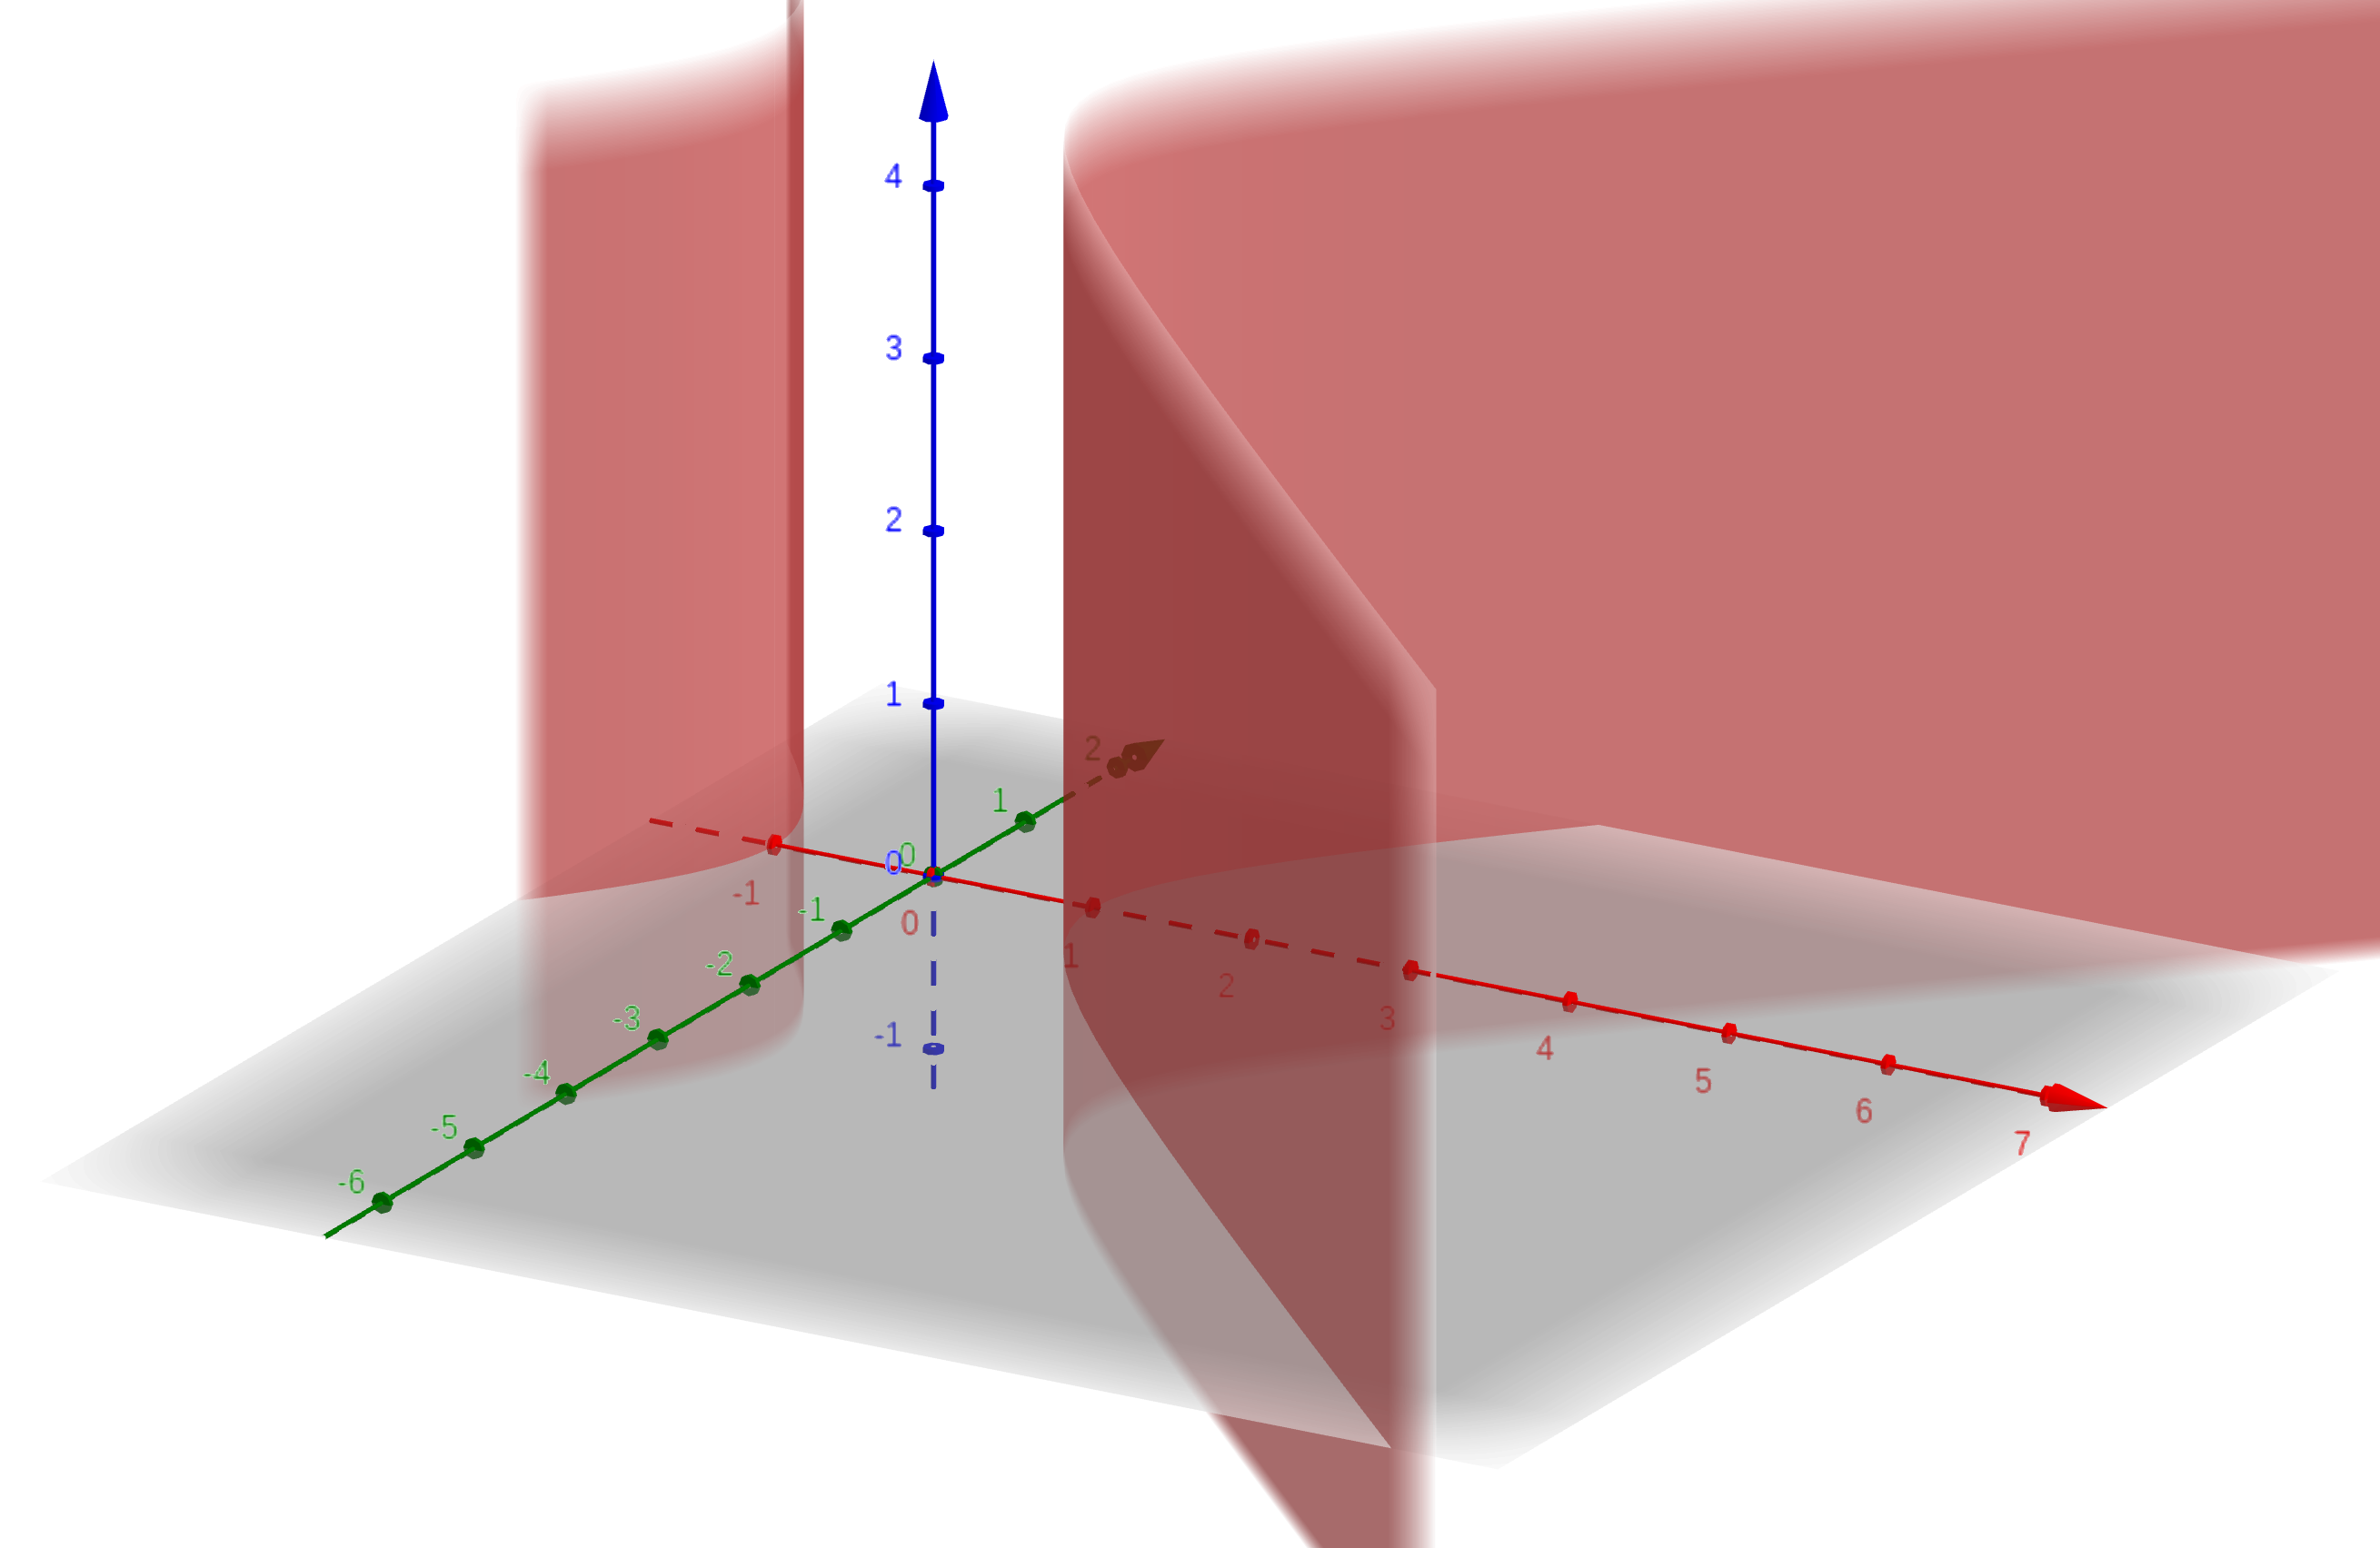
\includegraphics[width=\textwidth]{\svc/x^2-y^2=1(3d).png}
        \caption{Hyperbolisk cylinder $ax^2-by^2=1$, $a,b>0$}
    \end{subfigure}
       \caption{Geometriska object. Andra viktiga geometriska object är: Linje med normal (a,b) och Plan i $\mathbb{R}^3$ med normal (a,b,c).}
\end{figure}
\newpage

\section{Polära koordinater}
Beskriven en punkt i 2d.
\begin{equation*}
    x=r\cos(\theta), \; y=r\sin(\theta)
\end{equation*}
Där $r$ är avståndet från punkten till origo och $\theta$ är vinkeln till punkten.

\begin{figure}[H]
    \centering
    \includegraphics[width=5cm]{\svc/polär-koordinater.png}
    \caption{Polära koordinater}
\end{figure}


\section{Cylindriska koordinater}
Beskriven en punkt i 3d.
\begin{equation*}
    x=r\cos(\theta), \; y=r\sin(\theta), \; z
\end{equation*}
Dvs polär form med en viss höjd $z$

\begin{figure}[H]
    \centering
    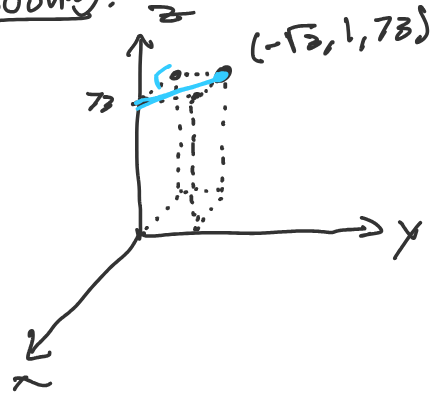
\includegraphics[width=5cm]{\svc/cylinder-koordinater.png}
    \caption{Cylinder koordinater}
\end{figure}


\section{Sfäriska koordinater}
\begin{equation*}
    x=R\cos(\theta)\sin{\phi}, \; y=R\sin(\theta)\sin(\phi), \; z=R\cos(\phi)
\end{equation*}

\begin{figure}[H]
    \centering
    \includegraphics[width=5cm]{\svc/sfäriska-koordinater.png}
    \caption{Sfäriska koordinater}
\end{figure}



\section{Parametriserade kurvor}
$\overline{r}(t) = (r_1(t), r_2(t), \ldots, r_n(t))$ där $r_n(t):[a,b] \to \mathbb{R}^n$.
Dvs en antal kontinuerliga funktioner som beskriver kurvan.

Där vi får hastighet $\overline{r}'(t)$, farten $||\overline{r}'(t)||$ och accelerationen $\overline{r}''(t)$.

\subsection{Några vanliga kurvor}
\textbf{En linje} med riktnings vektor $\overline{v}$ och start punkt $\overline{p}$.
\begin{equation*}
    \overline{r}(t) = \overline{p} + t\overline{v}
\end{equation*}


\textbf{En cirkel} med mittpunkt $(a,b)$ och radie $R$.
\begin{equation*}
    \overline{r}(t) = (a+R\cos(t), b+R\sin(t)), \; 0\leq t\leq 2\pi 
\end{equation*}

\section{Båglängd}
\textbf{Def:}
Båglängden (eller bara längden) $S$ av en kurva 
$\overline{r}:[a,b]\to\mathbb{R}^n$ är 
\begin{equation*}
    S = \int^{b}_{a} ||\overline{r}'(t)|| dt
\end{equation*}

%\textbf{Exempel:}
%$r(t) = (e^t\cos{t},e^t\sin{t})$, $0\leq t\leq2\pi$
%\textbf{Solution:}
%\begin{align*}
%    S = \int^{2\pi}_{0} || \overline{r}'(t) || dt
%\end{align*}
%\textbf{End of solution}


\section{Gränsvärden}

\subsection{Klämsatsen}
\textbf{Example:}
\begin{equation*}
    \lim_{(x,y)\to(0,0)} \frac{\sin(xy^2)}{xy}
\end{equation*}

\textbf{Solution:}
\begin{equation*}
    \left|\lim_{(x,y)\to(0,0)} \frac{\sin(xy^2)}{xy}\right| \leq  
    \lim_{(x,y)\to(0,0)} \frac{|xy^2|}{|xy|} = |y| \to 0
\end{equation*}
\textbf{End of solution:}


\subsection{Närma punkten från olika axlar}
\begin{itemize}
    \item Närma punkten via x-axeln
    \item Närma punkten via y-axeln
    \item Närma punkten via y är lika med punkten
\end{itemize}

\textbf{Example:}
\begin{equation*}
    \lim_{(x,y)\to(0,0)} \frac{x^2y^2}{x^4+y^4}
\end{equation*}

\textbf{Solution:}
Närmar origo från där $x=y$
\begin{equation*}
    \lim_{x\to0} \frac{x^2x^2}{x^4+x^4} = \frac{1}{2}
\end{equation*}

Närmar origo från x-axeln
\begin{equation*}
    \lim_{x\to0} \frac{x^2\cdot0}{x^4} = 0
\end{equation*}

Närmar origo från y-axeln
\begin{equation*}
    \lim_{y\to0} \frac{y^2\cdot0}{y^4} = 0
\end{equation*}

Dvs, gränsvädet existerar ej.
\textbf{End of solution:}


%\textbf{Example: TODO (2022-10-26 p2)}
%Visa att gränsvärdet $\lim_{(x,y)\to(0,0)}\frac{xy}{x^2+y^2}$ inte exsisterar.
%
%Närmar $(0,0)$ via x-axeln, dvs $\overline{r}(t)=(t,0)$.
%\begin{equation*}
%    \lim_{t\to0^+} f(\overline{r}(t)) = \lim_{t\to0^+} f(t,0) = \lim_{t\to0^+} \frac{t\cdot0}{t^2+0^2} = \lim_{t\to0^+} \frac{1\cdot0}{t} = 0
%\end{equation*}

\section{Partiella derivator}
Derivatan med avsende på $x$ av en funktion $f(x,y)$ i punkten $(a,b)$ defineras som
\begin{equation*}
    \frac{\partial f}{\partial x} (a,b) = \lim_{h\to0}\frac{f(a+h, b) - f(a,b)}{h}
\end{equation*}
och derivatan med acsende på x är en funktion $f(x,y)$ i punkten $(a,b)$ defineras som
\begin{equation*}
    \frac{\partial f}{\partial y} (a,b) = \lim_{h\to0}\frac{f(a, b+h) - f(a,b)}{h}
\end{equation*}

\textbf{Example:}
Låt $f(x,y) = x^2 + xy$, beräkna $\frac{\partial f}{\partial x}(1,2)$ och $\frac{\partial f}{\partial y}(1,2)$

\begin{align*}
    &\frac{\partial f}{\partial x}(x,y) = 2x + y \\
    &\frac{\partial f}{\partial x}(1,2) = 2 + 2 = 4
\end{align*}

\begin{align*}
    &\frac{\partial f}{\partial y}(x,y) = 0 + x \\
    &\frac{\partial f}{\partial y}(1,2) = 1
\end{align*}

\textbf{Tips:}\newline
Kvot regeln
\begin{equation*}
    f(x) = \frac{g(x)}{h(x)} \Leftrightarrow
    f'(x) = \frac{g'(x)h(x)-g(x)h'(x)}{(g(x))^2}
\end{equation*}

kedjeregeln
\begin{equation*}
    y(x) = f(g(x)) \Leftrightarrow
    y'(x) = f'(g(x))\cdot g'(x)
\end{equation*}



\section{Gradient}
Gradient till en funktion $f(\overline{x})$ i punkten $\overline{x}$ är 
vektorn som inehåller alla partiella derivator.
\begin{equation}
    \nabla f(\overline{x}) = \left( \frac{\partial f}{\partial x}(\overline{x}), \ldots, \frac{\partial f}{\partial x_n}(\overline{x}) \right)
\end{equation}

\textbf{Example:}
Berkäkna $\nabla f(1,2,3)$ då $f(x,y,z)=x^2+yz$

\textbf{Solution:}
\begin{equation*}
    \nabla f = \left( \frac{\partial f}{\partial x}, \frac{\partial f}{\partial y}, \frac{\partial f}{\partial z} \right)
    = (2x, z, y) \Rightarrow \nabla f(1,2,3) = (2,3,2)
\end{equation*}


\section{Deriverbarhet}
Vi säger att en envariable funktion $f:\mathbb{R}\to\mathbb{R}$ är deriverbar i en punkt 
$a$ med derivatan $f'(a)$ om
\begin{equation*}
    f(a+h) = f(a) + f'(a)h +R(n)
\end{equation*}
för någon funktion $R(n)$ sådan att
\begin{equation*}
    \lim_{h\to0} \frac{R(n)}{h} = 0
\end{equation*}

Alternativ definition av deriverbarhet.
Vi säger att $f:\mathbb{R}^n\supset D\to\mathbb{R}$ är deriverbar i 
en punkt $\overline{a} \in D$ om $\nabla f(\overline{a})$ exsisterar
och $f(\overline{a}+\overline{h}) = f(\overline{a}) + \nabla f(\overline{a})\cdot\overline{n} + R(\overline{n})$
för någon funktion $R(\overline{n})$ sådan att
\begin{equation*}
    \lim_{\overline{h}\to\overline{0}}\frac{R(\overline{n})}{||\overline{n}||} = 0
\end{equation*}

Med andra ord så har vi
\begin{equation*}
    \lim_{(h,k)\to(0,0)}\frac{f(x+h,y+k) - f(x,y) - \frac{\partial f}{\partial x}(x,y)h - \frac{\partial f}{\partial y}(x,y)k}{\sqrt{h^2+k^2}} = 0
\end{equation*}



\textbf{Example:}
Visa att $f(x,y) = \frac{x^4}{x^2+y^2}, (x,y) \neq (0,0)$ är deriverbar i hela $\mathbb{R}^2$.

\begin{align*}
    \frac{\partial f}{\partial x}(0,0) &= \lim_{h\to0}\frac{f(0+h, 0)-f(0,0)}{h} \\
    &= \lim_{h\to0}\frac{\frac{h^4}{h^2+0} - 0}{h} = 0 \\
\end{align*}

\begin{align*}
    \frac{\partial f}{\partial y}(0,0) &= \lim_{h\to0}\frac{f(0, 0+h)-f(0,0)}{h} \\
    &= \lim_{h\to0}\frac{\frac{0}{0^2+h} - 0}{h} = 0 \\
\end{align*}

\textbf{Sats:}
Om $f:\mathbb{R}^n\subset D \to\mathbb{R}$ är i klass $C^1$ så är funktionen deriverbar.

\subsection{Linjärisering}
\begin{equation*}
    L_{f,\overline{a}} (x_1,\ldots,x_n) = f(\overline{a}) 
    + \nabla f(\overline{a})\bullet(\overline{x}-\overline{a})
\end{equation*}

\textbf{Example:}
Hitta linjärisering till $f(x,y)=x^2y^2$ i punkten $(-2,1)$ samt tangentplanet till $z=x^2y^2$
i punkten $(-2,1,4)$.

\textbf{Lösning:}
\begin{align*}
    L_{f,(-2,1)}(x,y) &= f(-2,1) + \frac{\partial f}{\partial x}(-2,1)(x-(-2)) + \frac{f}{y}(-2,1)(y-1) \\
    f(-2,1) &= (-2)^2\cdot 1^2 = 4 \\
    \frac{\partial f}{\partial x} &= 2xy^2 \Rightarrow \frac{\partial f}{\partial x}(-2,1) = -4 \\
    \frac{\partial f}{\partial y} &= 2x^2y \Rightarrow \frac{\partial f}{\partial y}(-2,1) = 8 \\
    \Rightarrow L_{f,(-2,1)}(x,y) &= 4 -4(x+2) + 8(y-1) \\
\end{align*}
Tangentplanet i punkten $(-2,1,4)$ ges av $z=4 -4(x+2) + 8(y-1)$


\subsubsection{Linjär approximation}
Den exakta punkten $(a,b)$ kan approximeras med hjälp av punkten $(x,y)$
\begin{equation*}
    f(a,b) \approx f(x,y) + \frac{\partial f(a,b)}{\partial x}(x-a) + \frac{\partial f(a,b)}{\partial y}(y-b)
\end{equation*}

\textbf{Example:}
Bestäm närmvärdet till $f(1.01, 1.01)$ med hjälp av linjär approximation av $f$
kring $(1,1)$. Där $f(x,y) = 2\pi x + 2\pi y -4\pi$

\textbf{Lösning:}
\begin{align*}
    f(1.01,1.01) &= (2\pi +2\pi -4\pi) +(2\pi)(0.01) +(2\pi)(0.01) \\
    &= 0.04\pi
\end{align*}
\textbf{Slut på lösning}


\subsection{kedjeregeln}
\begin{align*}
    g'(t) &= \nabla f(\overline{r}(t))\bullet\overline{r}'(t) \\
    &= \frac{\partial f}{\partial x_1}(\overline{r}(t))\bullet\overline{r}'_1(t) + \ldots \frac{\partial f}{\partial x_n}(\overline{r}(t))\bullet\overline{r}'_n(t)
\end{align*}

\textbf{Example:}
Låt $f(x,y)=x^2+y^2$ och $\overline{r}(t)=(\cos{t},\sin{t})$ bilda en envariable funktion
$g(t)=f(\overline{t})$. Beräkna $g'(t)$.

\textbf{Lösning:}
\begin{align*}
    g'(t) &= \nabla f(\overline{r}(t))\bullet\overline{r}(t) = (2\cos(t), 2\sin(t)) \bullet (-\sin(t), \cos(t)) \\
    &= -2\cos(t)\sin(t) + 2\cos(t)\sin(t) = 0 \\
\end{align*}
\textbf{Alternativ:}
\begin{align*}
    g(t) &= f(\overline{r}(t)) = \cos^2t + \sin^2t = 1 \Rightarrow g'(t) = 0
\end{align*}


\subsection{Riktningsderivatan}
Låt $f:\mathbb{R}^n\subset D\to\mathbb{R}$, $\overline{a}\in D$.
Riktningsderivatan till $f$ i punkten $\overline{a}$ i riktning $\overline{v}\neq0$
beteknas med $D_{\overline{v}}f(\overline{a})$ och defineras med 
$D_{\overline{v}}f(a)=g'(0)=\nabla f(\overline{r}(0))\bullet\overline{r}'(0) = \nabla f(\overline{a})\bullet\frac{\overline{v}}{||\overline{v}||}$.

\begin{equation*}
    D_{\overline{v}}f(a)= \nabla f(\overline{a})\bullet\frac{\overline{v}}{||\overline{v}||}
\end{equation*}

\textbf{Example:}
Låt $f(x,y) = \sqrt{x^2+y^2}$ beräkna $D_{(3,4)}f(1,2)$

\textbf{Lösning:} 
\begin{align*}
    \nabla f &= \left( \frac{x}{\sqrt{x^2 + y^2}}, \frac{y}{\sqrt{x^2 + y^2}} \right) \\
    \nabla f(1,2) &= \left( \frac{1}{\sqrt{5}}, \frac{2}{\sqrt{5}} \right) \\
    D_{(3,4)}f(1,2) &= \left( \frac{1}{\sqrt{5}}, \frac{2}{\sqrt{5}} \right)\bullet\frac{(3,4)}{||(3,4)||} 
    = \frac{11}{5\sqrt{3}} \\
\end{align*}


\subsection{Geometriska egenskaper för gradienten}
\textbf{Sats:} 
Låt $f:\mathbb{R}^n\subset D\to\mathbb{R}$ vara deriverbar och 
$\overline{a}\in D$. Då är $\nabla f(\overline{a})$ den riktning
som $f$ växer snabbast i i punkten $\overline{a}$ och $-\nabla f(\overline{a})$
är den riktning som funktionen avtar snabbast i, i punkten $\overline{a}$.

Låt $f:\mathbb{R}^n\subset D\to\mathbb{R}$ och $\overline{a}\in D$.
Då är $\nabla f(\overline{a})$ vinkelrätt mot tangent (linje/plan)
till nivåmängden $f(\overline{x})=f(\overline{a})$ i punkten $\overline{a}$.


\section{Högre ordningens derivator}
\textbf{Example:} 
Beräkna alla andra ordningens derivator till 
$f(x,y) = e^{x^2y}$.

\textbf{Solution:} 
\begin{align*}
    &\frac{\partial f}{\partial x} = 2xye^{x^2y},\; \frac{\partial f}{\partial y} = x^2e^{x^2y} \\
    &\frac{\partial^2 f}{\partial x^2} = 2ye^{x^2y} + (2xy)(2xy)e^{x^2y} = (2y+4x^2y^2)e^{x^2y} \\
    &\frac{\partial^2 f}{\partial y\partial x} = 2xe^{x^2y} + (2xy)(x^2)e^{x^2y} = (2x+2x^3y)e^{x^2y} \\
    &\frac{\partial^2 f}{\partial x\partial y} = 2xe^{x^2y} + (x^2)(2xy)e^{x^2y} = (2x+2x^3y)e^{x^2y} \\
    &\frac{\partial^2 f}{\partial y^2} = (x^2)(x^2)e^{x^2y} = x^4e^{x^2y}
\end{align*}
Notera att $\frac{\partial^2 f}{\partial y\partial x} = \frac{\partial^2 f}{\partial x\partial y}$, vilket är fallet 
för många funktioner.
\textbf{End of solution:} 

\textbf{Def:} 
Låt $f: \mathbb{R}^n\subset D\to\mathbb{R}$. Om alla 
partiella derivator av ordningen $\leq K$ existerar 
och är kontinuerliga säger vi att $f$ är av klass $C^k$.
Om $f$ är av klass $C^k$ för alla $k<\infty$ säger vi att 
$f$ är av klass $C^\infty$.

\textbf{Anm:} 
Det flästa funktioner vi kommer kolla på är av klass $C^\infty$.

\textbf{Sats:} 
Om $f: \mathbb{R}^n\subset D\to\mathbb{R}$ är av klass $C^2$ 
så är $\frac{\partial^2 f}{\partial x_j\partial x_i} = \frac{\partial^2 f}{\partial x_i\partial x_j}$.

\subsection{Exempel på differentialekvationer}
Laplace ekvation i tree dimentioner lyder
\begin{equation*}
    \Delta f = \frac{\partial^2 f}{\partial x^2} + \frac{\partial^2 f}{\partial y^2} + \frac{\partial^2 f}{\partial z^2} = 0
\end{equation*}

Där $\Delta$ kallas för laplacianen.
Lösningen till en laplace ekvation kallas för harmoniska 
funktioner.

Laplace ekvation i två dimentioner lyder
\begin{equation*}
    \Delta f = \frac{\partial^2 f}{\partial x^2} + \frac{\partial^2 f}{\partial y^2} = 0
\end{equation*}

\textbf{Example:} 
Visa att funktionen $f = e^x \cos{y}$ är harmonisk.

\textbf{Solution:} 
\begin{align*}
    &\frac{\partial f}{\partial x} = e^x \cos{y} \\
    &\frac{\partial^2 f}{\partial x^2} = e^x \cos{y}
\end{align*}
\begin{align*}
    &\frac{\partial f}{\partial y} = -e^x \sin{y} \\
    &\frac{\partial^2 f}{\partial y^2} = -e^x \cos{y}
\end{align*}

\begin{align*}
    &\Delta f = \frac{\partial^2 f}{\partial x^2} + \frac{\partial^2 f}{\partial y^2} 
    = e^x \cos{y} -e^x \cos{y} =0
\end{align*}
\textbf{End of solution:} 


\section{Taylor polynom}
Från envariable analys 
\begin{equation*}
    f(x) = \underbrace{\sum^{n}_{k=0} \frac{f^{(k)}(a)}{k!}(x-a)^k}_{\text{taylorpolynom}} + \underbrace{\frac{f^{(n+1)}(c)}{(n+1)!}(x-a)^{(n+1)}}_{\text{rest term}} 
\end{equation*}

\textbf{Sats:} 
Om $f: \mathbb{R}^2\subset D \to\mathbb{R}$ är av klass $C^3$
och $(a,b)\in D$ så gäller.
\begin{align*}
    f(x,y) &= f(a,b) 
    +\frac{\partial f}{\partial x}(a,b)(x-a) 
    +\frac{\partial f}{\partial y}(a,b)(y-b) \\
    &+2!\left( 
    \frac{\partial^2 f}{\partial x^2}(a,b)(x-a)^2 
    +2\frac{\partial^2 f}{\partial y\partial x}(a,b)(x-a)(y-b)
    +\frac{\partial^2 f}{\partial y^2}(a,b)(y-b)^2 
    \right) \\
    &+\underbrace{B(x,y)||(x-a)(y-b)||^3}_{\text{Väldigt liten då } (a,b)\approx(x,y)}
\end{align*}

\textbf{Example:} 
Hitta taylorpolynomet (med restterm) av grad 2 i punkten $(2,3)$
till funktionen $f(x,y) = xy^2+x^2$.
\textbf{Solution:} 
\begin{align*}
    &f(2,3) = 2\cdot3^2+2^2 \\
    &\frac{\partial f}{\partial x} = y^2 + 2x,\; \frac{\partial f}{\partial x}(2,3) = 13 \\
    &\frac{\partial f}{\partial y} = 2xy,\; \frac{\partial f}{\partial y}(2,3) = 12 \\
    &\frac{\partial^2 f}{\partial x^2} = 2,\; \frac{\partial^2 f}{\partial x^2}(2,3) = 2 \\
    &\frac{\partial^2 f}{\partial x\partial y} = 2y,\; \frac{\partial^2 f}{\partial y^2}(2,3) = 6 \\
    &\frac{\partial^2 f}{\partial y^2} = 2x,\; \frac{\partial^2 f}{\partial y^2}(2,3) = 4
\end{align*}

\begin{align*}
    f(x,y) &= 22 + 13(x-2) + 12(y-3) \\
    &+\frac{1}{2!}(2(x-2)^2 +2\cdot3(x-2)(y-3) +4(y-3)^2) \\
    &B(x,y)\sqrt{(x-2)^2 +(y-3)^2}^3
\end{align*}
\textbf{End of solution:} 


\section{Kvadratiska former}
\textbf{Def:} En kvadratisk form på $\mathbb{R}^2$
funktion $Q: \mathbb{R}^2\to\mathbb{R}$ på formen
\begin{equation*}
    Q(h_1,\ldots,h_n) = \sum^{n}_{i,j=1} a_{ij}h_ih_j,\; a_{ij}\in\mathbb{R}
\end{equation*}

\textbf{Example:} 
Ekvationen
\begin{equation*}
    Q(h,k,l) = 2h^2 -4k^2 +5hl -kl
\end{equation*}
är en kvadratisk form.
Medans ekvationen
\begin{equation*}
    Q(h,k,l) = 5l^2 -\underbrace{k^3}_{\text{grad 3}} +\underbrace{2hl^2}_{\text{grad 3}} -\underbrace{h}_{\text{grad 1}} -\underbrace{3}_{\text{grad 0}}
\end{equation*}
är inte en kvadratisk form.

\textbf{Def:}
En kvadratisk form $Q:\mathbb{R}^n\to\mathbb{R}$ är
\begin{itemize}
    \item positivt definit $Q(\overline{h})>0$ $\forall\overline{h}\neq\overline{0}$
    \item negativt definit $Q(\overline{h})<0$ $\forall\overline{h}\neq\overline{0}$
    \item positivt semidefinit $Q(\overline{h})\geq0$ $\forall\overline{h}$
    \item negativt semidefinit $Q(\overline{h})\leq0$ $\forall\overline{h}$
    \item indefinit om $Q(\overline{h})$ antar både positiva och negativa värden.
\end{itemize}

\textbf{Example:} 
Avgör typen av den kvadratiska formen 
\begin{equation*}
    Q(h,k) = 2h^2 -8hk + 9k^2
\end{equation*}

\textbf{Solution:} 
\begin{align*}
    Q(h,k) &= 2(h^2 -4hk) + 9k^2 \\
    &= 2((h-2k)^2 -4k^2) + 9k^2 \\
    &= 2(h-2k)^2 +k^2 \\
\end{align*}
Dvs positivt definit eftersom $2(h-2k)^2 +k^2>0$ och $(h,k)\neq(0,0)$.
\textbf{End of solution} 


\subsection{Klassificering av kritiska punkter}
En kritisk punkt för funktionen $f:\mathbb{R}^n\subset D\to\mathbb{R}$
är $\nabla f(\overline{a})=\overline{0}$.

Punkten $\overline{x}$ är ett localt maximum om $f(\overline{x})>f(\overline{a})$,
$\forall\overline{a}$ närligande punkter kring $\overline{x}$.

Punkten $\overline{x}$ är ett localt minimum om $f(\overline{x})<f(\overline{a})$,
$\forall\overline{a}$ närligande punkter kring $\overline{x}$.

Punkten $\overline{x}$ är ett sadelpunkt om $f(\overline{x})<f(\overline{a})$
och $f(\overline{x})<f(\overline{a})$, 
$\forall\overline{a}$ närligande punkter kring $\overline{x}$.

\textbf{Sats:} 
Låt $f:\mathbb{R}^2\subset D\to\mathbb{R}$ vara av klass $C^2$
och $(a,b)\in D$ en kritisk punkt, definera den kvadratiska formen.
\begin{equation*}
    Q(h,k) = \frac{\partial^2 f}{\partial x^2}(a,b)h^2 + 2\frac{\partial^2 f}{\partial y\partial x}(a,b)hk +\frac{\partial^2 f}{\partial y^2}(a,b)k^2 
\end{equation*}
\begin{itemize}
    \item Om $Q$ är positivt definit är $(a,b)$ ett lokal minimum.
    \item Om $Q$ är negativt definit är $(a,b)$ ett lokal maximum.
    \item Om $Q$ är indefinit är $(a,b)$ en sadelpunkt.
\end{itemize}

\textbf{Example:} 
Hitta och bestäm typen av alla kritiska punkter till $f(x,y)=2x^3+3x^2y+2y^2+y$.
\textbf{Solution:} 
\begin{align*}
    \nabla f = \left( \frac{\partial f}{\partial x}, \frac{\partial f}{\partial y} \right) = (0,0)
    \begin{cases}
        \frac{\partial f}{\partial x} = 6x^2 +6xy = 0 \\
        \frac{\partial f}{\partial y} = 3x^2 +4y +1 = 0 \\
    \end{cases}
\end{align*}

\underline{Fall 1 $x=0$} Ekv 2 blir $4y+1=0\Leftrightarrow y=-\frac{1}{4}$
vi får den kritiska punkten $(0,\frac{1}{4})$.

\underline{Fall 2 $y=-x$} Ekv 2 blir $3x^2 -4x +1=0$
\begin{align*}
    \Leftrightarrow x^2 -\frac{4}{3}x +\frac{1}{3}=0
    \Leftrightarrow x= \frac{2}{3} \pm\sqrt{\frac{4}{9}-\frac{1}{3}}=0
    \Leftrightarrow x_1 = 1, x_2 = \frac{1}{3}
\end{align*}

\underline{Fall 1,2} så får vi det kritiska punkterna $(1,-1)$, $(\frac{1}{3}, -\frac{1}{3})$
och $(0,\frac{1}{4})$.

För att avgöra typen av punktenrna så behöver i alla derivator av ordning 2
\begin{equation*}
    \frac{\partial^2 f}{\partial x^2} = 12x + 6y,\; 
    \frac{\partial^2 f}{\partial xy} = 6x,\;
    \frac{\partial^2 f}{\partial y^2} = 4
\end{equation*}
Punkten $(0,-\frac{1}{4})$
\begin{equation*}
    Q(h,k) = -\frac{3}{2}h^2 + 2\cdot0hk + 4k^2 
\end{equation*}
är indefinit, $Q(1,0)=-\frac{3}{2}$, $Q(0,1)=4$ $\Rightarrow$ $(0,-\frac{1}{4})$ är en sadelpunkt.

Punkten $(1,-1)$
\begin{align*}
    Q(h,k) &= 6h^2 + 2\cdot6hk + 4k^2 \\
    &= 6(h^2 + 2hk) + 4k^2 \\
    &= 6((h+k)^2 -k^2) + 4k^2 \\
    &= 6(h+k)^2 -2k^2 \\
\end{align*}
Indefinit ($Q(1,0)=6$, $Q(1,1)=-2$) $\Rightarrow$ $(1,-1)$ är en sadelpunkt.

Punkten $(\frac{1}{3},-\frac{1}{3})$
\begin{align*}
    Q(h,k) &= 2h^2 + 2\cdot2hk + 4k^2 \\
    &= 2(h^2 + 2hk) + 4k^2 \\
    &= 2((h+k)^2 -k^2) + 4k^2 \\
    &= 2(h+k)^2 +2k^2 \\
\end{align*}
är störe än $(h,k)\neq(0,0)$ är positivt definit.

$\Rightarrow$ $(\frac{1}{3},-\frac{1}{3})$ är ett lokalt minimum.
\textbf{End of solution} 


\section{Optimering}

\textbf{Sats:} Om $f:\mathbb{R}^n\subset D\Rightarrow\mathbb{R}$ har minsta/största 
värde så antas det i någon av det följande typ av punkt
\begin{itemize}
    \item $\nabla f(\overline{x})=\overline{0}$
    \item $\overline{x}$ ligger på $\partial D$ (randen av $D$)
    \item där $f$ inte är deriverbar
\end{itemize}

\textbf{Sats:} Om $f:\mathbb{R}^n\subset D\Rightarrow\mathbb{R}$ är kontinuerligt
och $D$ är kompakt (slutet och begränsad) så antar $f$ både ett minsta och största 
värdet på $D$. 

\textbf{Example:} Låt $D=\{ (x,y)| x^2+y^2 \leq 1 \}$, $f: D\to\mathbb{R}$
$f(x,y)=\sqrt{x^2+y^2}$

\textbf{Solution:} är en kon vars minsta punkt är $(0,0)$.

\textbf{Example:} Avgör om funktion $f(x,y)=xy(x+2y-2)$ har ett minsta/största värde på området 
$0\leq x,y \leq 1$. Bestäm isåfall dessa värden.

\textbf{Solution:} Eftersom $f$ är kontinuerlig och området är kompakt så 
existerar både min och max. 

\textbf{steg 1:}
Vi undersöker området inre $0<x,y<1$ där $\nabla f(\overline{x})=(0,0)$.
\begin{align*}
    \begin{cases}
        0 = \frac{\partial f}{\partial x} = y(x+2y-2) +xy = y(2x+2y-2) \\
        0 = \frac{\partial f}{\partial y} = x(x+2y-2) +2xy = x(x+4y-2) \\
    \end{cases}
\end{align*}
Vi vet att $x\neq0$ and $y\neq0$ meaning that 
\begin{align*}
    \begin{cases}
        2x+2y = 2 \\
        x+4y-2 = 2 \\
    \end{cases}
\end{align*}
Då man man andvända gausselimination, och då får man
\begin{align*}
    x = \frac{2}{3} \\
    y = \frac{1}{3} \\
\end{align*}
Punkten $(\frac{2}{3}, \frac{1}{3})$ ligger i vårt omrdåde.
\begin{equation*}
    f\left(\frac{2}{3}, \frac{1}{3}\right) = -\frac{4}{27}
\end{equation*}

\textbf{steg 2:}
Vi undersöker områdets rand.
$x=0$, $0\leq y \leq1$ och där $y=0$, $0\leq x \leq1$ är funktionen $0$.

Där $x=1$, $0\leq y \leq1$ är
\begin{align*}
    &f(1,y) = y(2y-1) \\
    &f(1,0) = 0, f(1,1) =1 \\
\end{align*}
Vi undersöker där derivatan är $0$
\begin{align*}
    &\frac{\partial f}{\partial y}(1,y) = 4y-1 = 0 \Leftrightarrow y = \frac{1}{4} \\
    &f\left(1,\frac{1}{4}\right) = \frac{1}{4}\left(2\frac{1}{4} - 1\right) = -\frac{1}{8} 
\end{align*}
Vilket inte är det minsta värdet.

Där $y=1$, $0\leq x \leq1$ är
\begin{align*}
    &f(x,1) = x(x) = x^2, 0\leq x \leq1 \\
    &\frac{\partial f}{\partial x}(x,1) = 2x = 0 \Leftrightarrow x = 0
\end{align*}
antar minsta värdet det $x=0$ då är $f(0,1) = 0$ och största värdet då
$x=1$ då är $f(1,1)=1$.

\textbf{Svar:} min är $-\frac{4}{27}$ och antas i $(\frac{2}{3}, \frac{1}{3})$,
max är $1$ och antas i $(1,1)$.

\textbf{End of solution}


\subsection{Optimering med bivilkor}

\textbf{Sats:}
Om deriverbara funktionen $f$ antar ett minsta/största värde på en nivåmängd
$g=c$ där $g$ är deriverbar, så kommer det att antas i en punkt $\overline{a}$
där $\nabla f(\overline{a}) || g(\overline{a})$, dvs parallel med bivilkoret.

\textbf{Example:}
Hitta punkten som från klotet $x^2+y^2+z^2=16$ som är närmast origo.

\textbf{Solution:}
Låt avståndet mellan origo och funktionen vara $a$
\begin{equation*}
    \sqrt{x^2+y^2+z^2} = a \Leftrightarrow
    x^2+y^2+z^2 = a^2
\end{equation*}
Vi vill minimera $a$ för att få den punkt som närmast origo. 
Låt $f(x,y,z)=x^2+y^2+z^2$.
Vi använder den som vår givna funktion vara vårt bivillkor 
$g(x,y,z)=x^2+y^2+z^2=16$.

Vi vill ta reda på när bivillkor är parallellt med vår funktion, 
dvs $\nabla f(x,y,z) || \nabla g(x,y,z)$.
\begin{align*}
    &\nabla f(x,y,z) = (2x,2y,2z) \\
    &\nabla g(x,y,z) = (10x-6y, 10y-6x, 2z)
\end{align*}

\begin{align*}
    &\begin{cases}
        2x = \lambda (10x-6y) \\
        2y = \lambda (10y-6x) \\
        2z = \lambda 2z
    \end{cases}
\end{align*}
Antigen är $z=0$ och då får $\lambda$ ha ett giltigt värde, annars så är $\lambda = 1$ då $z\neq0$.

\textbf{Fall 1:} $z\neq0$
\begin{align*}
    &\begin{cases}
        x = \lambda (5x-3y) \\
        y = \lambda (5y-3x) \\
        \lambda = 1
    \end{cases} \\
    &\begin{cases}
        4x = 3y \\
        4y = 3x \\
    \end{cases}
    \begin{cases}
        x = \frac{3}{4}y \\
        x = \frac{4}{3}y  \\
    \end{cases} \\
    & \frac{3}{4}y = \frac{4}{3}y \Leftrightarrow y = 0
\end{align*}
Vilket är endast fallet då $x=y=0$ och $z$ får anta giltigt värde.

\begin{align*}
    &g(x,y,z) = 5\cdot0^2 + 5\cdot0^2 + z^2 -6\cdot 0 \cdot 0 = 16 \\
    &\Leftrightarrow z = \pm \sqrt{16} = \pm 4
\end{align*}
Dvs så har vi ett par kritiska punkter $(0,0,\pm4)$.

\textbf{Fall 2:} $z=0$
\begin{align*}
    &\begin{cases}
        x = \lambda (5x-3y) \\
        y = \lambda (5y-3x) \\
    \end{cases} 
    \Rightarrow \lambda = \frac{x}{5x-3y} \\
    &y = \frac{x}{5x-3y} (5y-3x) \\
    &y(5x-3y) = x(5y-3x)  \\
    &5xy-3y^2 = 5yx-3y^2  \\
    &y^2 = x^2  \\
    &x = \pm y 
\end{align*}

\textbf{Beräknar punkterna för} $(x,y,0) = (x,x,0)$
\begin{align*}
    &5x^2+5x^2 -6x^2 = 16 \\
    &4x^2 = 16 \\
    &x^2 = 4 \\
    &x = \pm2
\end{align*}

\textbf{Beräknar punkterna för} $(x,y,0) = (x,-x,0)$
\begin{align*}
    &5x^2+5(-x)^2 +6x^2 = 16 \\
    &16x^2 = 16 \\
    &x = \pm\sqrt{1} = \pm1
\end{align*}

\textbf{Tar reda på min och max av det kritiska punkterna}
\begin{align*}
    &f(0,0,-4) = f(0,0,4) = 0^2 + 0^2 + 4^2 = 16 \\
    &f(-2,2,0) = f(2,2,0) = 2^2 + 2^2 + 0^2 = 8 \\
    &f(1,-1,0) = f(-1,1,0) = (-1)^2 + 1^2 + 0^2 = 2 \\
\end{align*}

\textbf{Svar}: De punkter som är längs ifrån origo är $(0,0,\pm4)$ ($4$ enheter från origo).
De punkter som är närmast origo är $(1,-1,0)$ och $(-1,1,0)$ ($\sqrt{2}$ enheter från origo).


\textbf{End of solution}


\section{Dubble integraler}

\textbf{Def:} En funktion $f(x,y)$ är 
\begin{itemize}
    \item udda map $x$ om $f(-x,y) = -f(x,y)$
    \item jämn map $x$ om $f(-x,y) = f(x,y)$
    \item udda map $y$ om $f(x,-y) = -f(x,y)$
    \item jämn map $y$ om $f(x,-y) = f(x,y)$
\end{itemize}

\textbf{Sats:}
Om $D\subset\mathbb{R}^2$ är symetrisk map $x$ och $f(x,y)$ är udda map $x$
så är $\iint_D f(x,y)dxdy = 0$ om $D\subset\mathbb{R}^2$ är symetrisk map $y$
och map $y$ och $f(x,y)$ är udda map $y$ så är $\iint_D f(x,y)dxdy = 0$.

\textbf{Example}
\begin{align*}
    &\iint\limits_{x^2+y^2\leq 2^2} 6-x^2-y^2 dxdy 
    =\iint\limits_{\substack{0\leq r\leq2 \\ 0\leq\theta\leq2\pi}} (6-r^2) rdrd\theta 
    =\iint\limits_{\substack{0\leq r\leq2 \\ 0\leq\theta\leq2\pi}} 6r-r^3 drd\theta \\
    &=\left(\int^{\theta=2\pi}_{\theta=0}1d\theta\right) \left(\int^{r=2}_{r=0} 6r-r^3dr\right)  
    =2\pi \left[ 3r^2-\frac{1}{4}r^4 \right]^{2}_{0} \\
    &=2\pi (3\cdot2^2-\frac{1}{2^2}2^4) = 2^3\pi(3-1) = 16\pi
\end{align*}



%\subsection{Axelparallella rektanglar}
%TODO: y-enkelt

\subsection{Variabelbyte}
Låt $x = x(u,v)$, $y=y(u,v)$ vara en $C^1$ och bijektiv avbildning från
området $E$ i $uv$-planet till området $D$ i $xy$-planet.

\begin{figure}[H]
    \centering
    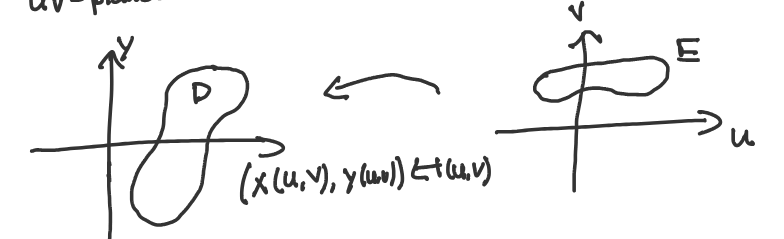
\includegraphics[width=8cm]{\svc/variabelbyte.png}
    \caption{vektorfält}
\end{figure}



Då är $\iint_D f(x,y)dxdy = \iint_E f(x(u,v), y(u,v))\left| \frac{\partial (x,y)}{\partial (u, v)}dudv\right|$
Där skalfaktorn 
\begin{equation*} 
    \left| \frac{\partial (x,y)}{\partial (u, v)}dudv\right| 
    = \left|\det\begin{bmatrix} \frac{\partial x}{\partial u} & \frac{\partial x}{\partial v} \\ \frac{\partial y}{\partial u} & \frac{\partial y}{\partial v} \end{bmatrix}\right|
\end{equation*} 
dvs absolutbelopet av determinaten av jacobimatrisen.

\textbf{Example:}
Skalfaktorn för polära koordinater ger 
\begin{equation*} 
    dxdy = rdrd\theta
\end{equation*} 

\subsection{Medelvärde}
Medelvärde av en funktion $f(x,y)$ på ett område $D$ ges av
\begin{equation*}
    \left( \iint_D f(x,y)dxdy \right) / \text{Arean}(D) 
\end{equation*}


\section{Generaliserad integraler}
\textbf{Def:} En dubbleintegral $\iint_D f(x,y)dxdy$ kallas 
generaliserad om antigen $D\subset\mathbb{R}^2$ är obegränsad 
eller om $f(x,y)$ är obegränsad på $D$.

\textbf{Def:} Låt $D\subset\mathbb{R}^2$ och $f(x,y) \geq 0$ på 
$D$ (eller $f(x,y)leq0$ på $D$). Låt $D_1\subset D_2\subset D_3 \ldots \subset D_n \subset\mathbb{R}^2$
vara en följd av begränsade omrdåden sådanna att $U^{\infty}_{n=1} = D$
och $f(x,y)$ är begränsad på alla omdråden $D_n$. Då definerar vi
\begin{equation*}
    \iint_D f(x,y)dxdy = \lim_{n\to\infty} \iint_{D_n} f(x,y)dxdy
\end{equation*}

TODO: Example


\section{Trippelintegraler}
\begin{equation*}
    \text{Volym}(D) = \iiint_D dxdydz
\end{equation*}


Några linjäritets egenskaper
\begin{align*}
    &\iiint_D \left(f(x,y,z) \pm g(x,y,z)\right)dxdydz 
    =\iiint_D f(x,y,z) dxdydz \pm \iiint_D g(x,y,z) \\
    &\iiint_D \alpha f(x,y,z) dxdydz 
    = \alpha \iiint_D f(x,y,z) dxdydz,\; \alpha \in \mathbb{R}
\end{align*}

Finns två sätt att lösa en trippelintegral med itererad integration
\textbf{enkelintegrera ytters} och \textbf{dubbleintegrera ytters}.

\textbf{Example: enkelintegrera ytters}
Beräkna 
\begin{equation*}
    \iiint\limits_{\substack{x^2+y^2-z^2\leq1 \\ 0\leq z\leq1}}(x+y+z)dxdydz
\end{equation*}

\textbf{Solution:}
Symetrisk med avsende på x och y
\begin{align*}
    &\iiint\limits_{\substack{x^2+y^2-z^2\leq1 \\ 0\leq z\leq1}}(z)dxdydz \\
    &=\int^{z=1}_{z=0}\left(\iint\limits_{x^2+y^2\leq 1+z^2} zdxdy\right) dz \text{ dvs cirkelns radie är} \sqrt{1+z^2} \\
    &=\int^{z=1}_{z=0} z\pi(1+z^2) dz =\pi\int^{z=1}_{z=0} z+z^3 dz \\
    &=\pi\left[ \frac{z^2}{2} + \frac{z^4}{4} \right]^{z=1}_{z=0} = \frac{3\pi}{4} \\
\end{align*}
\textbf{End of solution}


\textbf{Example: dubbleintegrera ytters}
Beräkna 
\begin{equation*}
    \iiint\limits_{\substack{0\leq z\leq 1+x^2-y^2 \\ x^2+y^2\leq 1}}(x+y+1)dxdydz
\end{equation*}

\textbf{Solution:}
Symetrisk med avsende på x och z (rita bild först)
\begin{align*}
    &\iint\limits_{x^2+y^2\leq1}\left(\int^{z=1+x^2-y^2}_{z=0}1dz\right) dxdy \\
    &=\iint\limits_{x^2+y^2\leq1}1+x^2-y^2 dxdy \\
    &=\text{Area}(x^2+y^2\leq1) = \pi
\end{align*}
\textbf{End of solution}



\subsection{Variabelbyte}
\textbf{sats:} Låt $x=x(u,v,w)$, $y=y(u,v,w)$, $z=z(u,v,w)$ vara en $C^1$ och bijektiv
av bildningen D i xyz-rummet. Då är 
\begin{equation*}
    \iiint\limits_{D} f(x,y,z)dxdydz = 
    \iiint\limits_{E} f(x(u,v,w),y(u,v,w),z(u,v,w)) \underbrace{\left| \frac{\partial(x,y,z)}{\partial(u,v,w)} \right|}_{\text{skalfaktorn}} dudvdw
\end{equation*}
där 
\begin{equation*}
    \left| \frac{\partial(x,y,z)}{\partial(u,v,w)} \right| 
    = \left|\det
    \underbrace{
    \begin{bmatrix} 
        \frac{\partial x}{\partial u} & \frac{\partial x}{\partial v} & \frac{\partial x}{\partial w} \\
        \frac{\partial y}{\partial u} & \frac{\partial y}{\partial v} & \frac{\partial y}{\partial w} \\
        \frac{\partial z}{\partial u} & \frac{\partial z}{\partial v} & \frac{\partial z}{\partial w}
    \end{bmatrix}}_{\text{jacobimatrisen}}\right|
\end{equation*}

Ett viktigt variable byte för trippelintegraler är sfäriska koordinater.
\textbf{Sats:} För sfäriska koordinater
\begin{equation*}
    \begin{cases}
        x=R\cos\theta\sin\phi \\ 
        y=R\sin\theta\sin\phi \\ 
        z=R\cos\phi \\ 
    \end{cases}
\end{equation*}
ger skalfaktorn $|\frac{\partial(x,y,z)}{\partial(R,\phi,\theta)}| = R^2\sin\phi$


\section{Vektorfält}
\textbf{Def:} Ett vektorfält på ett område $D\subset\mathbb{R}^n$
är en function $\overline{F}:D\to\mathbb{R}^n$. Ofta beteknas vektorfält
med dess komponenter $F_1,F_2,\ldots,F_n$ där
\begin{equation*}
    \overline{F}(x_1,\ldots,x_n) = \left(F_1(x_1,\ldots,x_n),\ldots,F_n(x_1,\ldots,x_n)\right)
\end{equation*}

\begin{figure}[H]
    \centering
    \includegraphics[width=\textwidth]{\svc/vektorfält.png}
    \caption{vektorfält}
\end{figure}


\subsection{Fältlinje}
En kurva $\overline{r}:[a,b]\to D\subset\mathbb{R}^n$ som hela tiden har samma
hastighet som ett väktorfält $\overline{F}$, dvs $\overline{r}'=\overline{F}(\overline{r})$ .
kallas för en fältlinje eller integralkurva till $\overline{F}$.

\textbf{Example:}
Visa att $\overline{r}(t) = (ae^{t/2},be^{t/2}),\;a,b\in\mathbb{R}$ är fältlinjer
till till $\overline{F} = \left(\frac{x}{2},\frac{y}{2}\right)$.

\textbf{Solution}
\begin{align*}
    &\text{VL} = \overline{r}' = \left(\frac{a}{2}e^{t/2}, \frac{b}{2}e^{t/2}\right) \\
    &\text{HL} = \overline{F}(\overline{r}) = \overline{F}((ae^{t/2},be^{t/2})) = \left(\frac{a}{2}e^{t/2}, \frac{b}{2}e^{t/2}\right)
\end{align*}
Eftersom HL=VL så är $\overline{r}$ en fältlinje.

\textbf{End of solution}


\subsection{Konservativa vektorfält}
\textbf{Def:} Ett vektorfält $\overline{F}=\mathbb{R}^n\supset D\to\mathbb{R}^n$
som uppfyller $\overline{F}=\nabla\phi$ för någon funktion $\phi:D\to\mathbb{R}$
kallas konservativt. Funktionen $\phi$ kallas för en potential till $\overline{F}$.

\textbf{Sats:} Om ett vektorfält $\overline{F}: \mathbb{R}^n\supset D\to\mathbb{R}^n$
är konservativt och klass $C^1$ så gäller.
\begin{equation*}
    \frac{\partial F_i}{\partial x_j}
    = \frac{\partial F_j}{\partial x_i}
\end{equation*}
för $1\leq i,j \leq n$

\textbf{Example:}
Vektorfält $\overline{F}(x,y) = (-5y, 5x)$ är inte konservativ eftersom
\begin{equation*}
    \frac{\partial F_1}{\partial y} = -5,\; \frac{\partial F_2}{\partial x} = 5
\end{equation*}

\textbf{Example:}
Är vektorfält $\overline{F}(x,y) = (y\sin x, \sin y - \cos x)$ konservativ? 
Hitta isåfall en potential $\phi:\mathbb{R}^2\to\mathbb{R}$ så att $\nabla \phi = \overline{F}$.

\textbf{Solution}
Kolla först om den är konservativ. Då ser man att den är det.


\begin{align*}
    &\left(\frac{\partial \phi}{\partial x}, \frac{\partial \phi}{\partial y} \right) = (F_1, F_2)
    &\begin{cases}
        \frac{\partial \phi}{\partial x} = y\sin x \\
        \frac{\partial \phi}{\partial y} = \sin y - \cos x
    \end{cases}
\end{align*}
Om vi andvänder ekv 1 så får vi $\phi = -y\cos x + f(y)$.
Och med ekv 2 så får vi att 

\begin{align*}
    &\frac{\partial \phi}{\partial y} = -\cos x + f'(y) \Rightarrow f'(y) = \sin y \\
    &\Rightarrow f(y) = -\cos y + C \\
    &\Rightarrow \phi(x,y) = -y\cos x - \cos y \\
\end{align*}
\textbf{End of solution}



\section{Kurvintegraler}
\textbf{Def:} Låt $\overline{F}:\mathbb{R}^n \supset D\to\mathbb{R}^n$ vara ett
vektorfält och $\mathcal{C}$ en kurva i $D$ Parametriserad av $\overline{r}:[a,b]\to D$.
Då definerar vi kurvintegralen av $\overline{F}$ längs $\mathcal{C}$ med formen
\begin{equation*}
    \int_{\mathcal{C}} \overline{F} \bullet d\overline{r} = \int^{b}_{a} \overline{F}(\overline{r}(t)) \bullet \overline{r}'(t)dt
\end{equation*}

\textbf{Example:} Beräkna $\int_{\mathcal{C}} xydx - (x+y)dy$ från $\mathcal{C}$
är kurvan från $(0,0)$ till $(2,4)$ längs parabeln $y=x^2$.

\textbf{Solution}
Vi parametriserar kurvan $\overline{r}(t) = (t,t^2),\; 0\leq t\leq 2$, $\overline{r}'(t) = (1,2t)$
\begin{align*}
    &\int^{2}_{0} \overline{F}(\overline{r}(t)) \bullet \overline{r}'(t)dt \\
    &=\int^{2}_{0} (t\cdot t^2, -t -t^2) \bullet (1,2t)dt \\
    &=-\frac{28}{3}
\end{align*}
\textbf{End of solution}

\subsection{Kurvintegraler av konservativa vektorfält}

\textbf{Sats:} Om $\overline{F} = \nabla\phi$ är konservativt vektorfält på 
$D\subset\mathbb{R}^n$ och $\mathcal{C}$ är en kurva i $D$ så är
\begin{equation*}
    \int_{\mathcal{C}} \overline{F}\bullet d\overline{r} = \phi(\text{slutpunkt}) - \phi(\text{startpunkt})
\end{equation*}

\textbf{Example:}
Beräkna $\int_{\mathcal{C}} 2xy^3dx + 3x^2y^2dy$ där $\mathcal{C}$ är en
godtycklig kurva från $(-1,-1)$ till $(3,2)$

\textbf{Solution}
Vi försöker hitta $\phi$ så att $\nabla\phi=\overline{F}$, dvs
\begin{align*}
    &\begin{cases}
        \frac{\partial\phi}{\partial x} = 2xy^3
        \frac{\partial\phi}{\partial y} = 3x^2y^2
    \end{cases} \\
    &\phi(x,y) = x^2y^3 + f(y) \\
    &\frac{\partial\phi}{\partial y} x^2y^3 + f(y) = 3x^2y^2 \\
    &\Rightarrow f(y) = C \Rightarrow \phi = x^2y^3 \text{ väljer } C=0
\end{align*}

Eftersom den är konservativ så kan vi
\begin{align*}
    &\int_{\mathcal{C}} \overline{F}\bullet d\overline{r} = \phi(3,2) - \phi(-1,-1) \\
    &= 3^2\cdot2^3 - (-1)^2\cdot(-1)^3 = 6\cdot8 + 1 = 49 \\
\end{align*}
\textbf{End of solution}


\subsection{Greens sats}
\textbf{Sats:} Låt $D\subset\mathbb{R}^2$ vara ett område med rand $\partial D$ 
(med området $D$ på vänster sida) som är styckvis av klass $C^1$ och $\overline{F}:D\to\mathbb{R}^2$
ett vektrofält av klass $C^1$. Då är 
\begin{equation*}
    \oint_{\partial D} \overline{F}\bullet d\overline{r} = \iint_{D} \left(\frac{\partial F_2}{\partial x} - \frac{\partial F_1}{\partial y}\right)dxdy
\end{equation*}

\textbf{Example:}
Beräkna $\int_{\mathcal{C}} \overline{F}\bullet d\overline{r}$ där $\mathcal{C}$
är delen av enhetscirkeln i första kvadraten från $(1,0)$ till $(0,1)$ och 
$\overline{F}=(e^x +1, 4x + y)$. 

\textbf{Solution}
Enlight greens sats

Rita bild och rita ut $\gamma_2$ från $(0,0)$ till $(0,1)$ och $\gamma_1$ $(0,0)$ till $(1,0)$.
Och $D$ är området som omringas.
\begin{align*}
    &\underbrace{\int_{\mathcal{C}} \overline{F}\bullet d\overline{r}}_{\text{vill veta men är svårt}} 
    -\int_{\gamma_2} \overline{F}\bullet d\overline{r} 
    +\int_{\gamma_1} \overline{F}\bullet d\overline{r} 
    \stackrel{\text{green}}{=} \iint_{D} \left(\frac{\partial F_2}{\partial x} - \frac{\partial F_2}{\partial y}\right) \\
    &\iint_{D} 4 dxdy = 4\text{Arean}(D) = \pi \\
\end{align*}
Parametriserar $\gamma_1$ med $\overline{r} = (t,0)$, $0\leq t \leq 1$
\begin{align*}
    &\int_{\gamma_1} \overline{F}\bullet d\overline{r} = \int^{1}_{0} (e^t+1, 4t + 0)\bullet(1,0) dt \\
    &= \int^{1}_{0} e^t+1 dt = \left[ e^t+t \right]^{1}_{0} = e+1-1 = e \\
\end{align*}

Parametriserar $\gamma_2$ med $\overline{r} = (0,t)$, $0\leq t \leq 1$
\begin{align*}
    &\int_{\gamma_2} \overline{F}\bullet d\overline{r} = \int^{1}_{0} (e^0+1, 4\cdot0 + t)\bullet(0,1) dt \\
    &=\int^{1}_{0} t dt = \left[ \frac{t^2}{2} \right]^{1}_{0} = \frac{1}{2} \\
\end{align*}

Kan vi ta reda på den svåra integrallen 
\begin{align*}
    &\int_{\mathcal{C}} \overline{F}\bullet d\overline{r}
    =+\iint_{D} \left(\frac{\partial F_2}{\partial x} - \frac{\partial F_2}{\partial y}\right)
    +\int_{\gamma_2} \overline{F}\bullet d\overline{r}
    -\int_{\gamma_1} \overline{F}\bullet d\overline{r} \\
    &= \pi + e - \frac{1}{2} \\
\end{align*}
\textbf{End of solution}


\subsection{Area beräkning med Greens sats}

\begin{align*}
    \text{Area}(D) &= \iint_{D}dxdy \stackrel{\text{green backlänges}}{=} \oint_{D} (0,x)\bullet d\overline{r} \\
    \text{Area}(D) &= \iint_{D}dxdy \stackrel{\text{green backlänges}}{=} \oint_{D} (-y,0)\bullet d\overline{r} \\
    \text{Area}(D) &= \iint_{D}dxdy \stackrel{\text{green backlänges}}{=} \oint_{D} \left(-\frac{y}{2},\frac{x}{2}\right)\bullet d\overline{r} \\
\end{align*}

\textbf{Example:}
Hitta arean av området som begränsas av kurvan $\overline{r}(t)=(a\cos^3t,b\sin^3t)$,
$0\leq t \leq 2\pi$, $a,b\in\mathbb{R}$

\textbf{Solution}
\begin{align*}
    \text{Area}(D) \stackrel{\text{green backlänges}}{=}& 
    \frac{1}{2} \oint_{\partial D} (-y,x)\bullet d\overline{r} 
    =\frac{1}{2} \oint^{2\pi}_{0} (-b\sin^3t,a\cos^3t)\bullet d\overline{r}' dt
\end{align*}

\textbf{End of solution}


\section{Kom ihåg}
\textbf{Parametrisera: Polära koordinater}
Eftersom vi har en cirkel så vet vi att $x^2+y^2=r^2$.
$x=r\cos(\theta)$ och $y=r\sin{theta}$. Vi har att $dxdy=rdrd\theta$

\textbf{Parametrisera: Cylindriska koordinater}
$r\in[0,\text{radie}]$, $\theta\in[0,2\pi]$ och $z=z$ med interval tas fram från 
$x=r\cos(\theta)$ och $y=r\sin{theta}$. Vi har att $dxdydz=rdrdzd\theta$

\textbf{Parametrisera: Sfäriska koordinater}
$x=r\cos(\theta)\sin(\phi)$, $y=r\sin(\theta)\sin(\phi)$ och $z=R\cos{\phi}$. Vi har att $dxdy=r^2\sin(\phi)drd\theta$


\textbf{Linjärisering}
\begin{equation*}
    L_{f,\overline{a}} (x_1,\ldots,x_n) = f(\overline{a}) 
    + \nabla f(\overline{a})\bullet(\overline{x}-\overline{a})
\end{equation*}


\textbf{Riktningsderivatan}
\begin{equation*}
    D_{\overline{v}}f(\overline{a})= \nabla f(\overline{a})\bullet\frac{\overline{v}}{||\overline{v}||}
\end{equation*}


\textbf{Deriverbarhet}
\begin{equation*}
    \lim_{(h,k)\to(0,0)}\frac{f(x+h,y+k) - f(x,y) - \frac{\partial f}{\partial x}(x,y)h - \frac{\partial f}{\partial y}(x,y)k}{\sqrt{h^2+k^2}} = 0
\end{equation*}
Kan också skrivas
\begin{equation*}
    \lim_{(x,y)\to(a,b)}\frac{f(x,y) - f(a,b) - \frac{\partial f(a,b)}{\partial x}(x-a) - \frac{\partial f(a,b)}{\partial y}(y-b)}{\sqrt{(x-a)^2+(y-b)^2}} = 0
\end{equation*}


\textbf{Trigonometriska regler}
\begin{equation*}
    \lim_{x\to0} |\sin(x)| \leq |x|
\end{equation*}
\begin{equation*}
    \sin^2\theta + \cos^2\theta = 1
\end{equation*}


\textbf{Greens sats}
\begin{equation*}
    \oint_{\partial D} \overline{F}\bullet d\overline{r} = {\color{red}-} \iint_{D} \left(\frac{\partial F_2}{\partial x} - \frac{\partial F_1}{\partial y}\right)dxdy
\end{equation*}

\textbf{Greens backlänges}
Är bra för att beräkna arean för ett område som den slutna kurvan skapar.


\textbf{Andra grads integral utan ekvation är arean}
\begin{equation*}
    \iint_{D} dxdy = \text{Area}(D)
\end{equation*}


\textbf{Udda och symetrisk}
Om vi har ett ett definitions omdråde som vi integrerar ifrån och det området 
är exempelvis \textit{symetrisk map x} och integralen så finns det termer som är 
\textit{udda map x} så kan man ta bort dem för det kommer ta ut varandra.

\textbf{Kurvintegraler}
\begin{equation*}
    \int_{\mathcal{C}} \overline{F} \bullet d\overline{r} = \int^{b}_{a} \overline{F}(\overline{r}(t)) \bullet \overline{r}'(t)dt
\end{equation*}


\textbf{Primitiva funktioner}
\begin{align*}
    &\sin^2\theta \Rightarrow \frac{\theta}{2} - \frac{\sin2\theta}{4}, 
    &\cos^2\theta \Rightarrow \frac{\theta}{2} + \frac{\sin2\theta}{4} \\
    &\frac{1}{x} \Rightarrow \ln{x}, &\ln{x} \Rightarrow x\ln{x}-x
\end{align*}


